
Este capítulo tem como objetivo apresentar o detalhamento da implementação dos subsistemas do \textit{r2-pi2}. Ao longo do capítulo será possível analisar estratégias de solução, equipamentos utilizados, tecnologias incorporadas e o resultado obtido durante a segunda fase de desenvolvimento do projeto R2-PI2.

% 
\section{Alimentação} % (fold)
\label{sec:alimentação}
	
	O sistema de alimentação pode ser dividido em 2 grandes grupos: \textit{Bateria} e \textit{Carregador}, os quais estão descritos nas sub-seções dispostas a seguir.

	\subsection{Bateria de íon-lítio (Li-Ion)} % (fold)
	\label{sub:bateria}
		
		De todos os tipos de baterias esta é, sem dúvida, a melhor. Suas vantagens são diversas e variadas e não é justamente por isso que elas são empregadas em larga escala nos novos eletrônicos.

		Não-tóxicas, com capacidade de carga duas vezes maior que as de Ni-MH e três vezes maior que as de NiCd, sem efeito memória (ou seja, a bateria não vai “viciar”) e também mais leves, afinal o lítio é um dos metais mais leves já conhecidos. A densidade do lítio também permite a criação de baterias com maior capacidade.

		Outro ponto que dá muito mais vantagens às baterias de Li-Ion é o fato de estas baterias dispensarem ciclos completos de cargas, ou seja, não é necessário esperar a carga acabar para carregá-la novamente e quando carrega não precisa esperar que ela seja preenchida por completo. Além disso, ao estar carregada por completo a bateria cessa automaticamente o recebimento de energia para evitar sobrecargas.

		Estas baterias, porém, demandam um cuidado maior por parte de seus usuários, como por exemplo, a não exposição a altas temperaturas que podem causar danos definitivos e até mesmo sua explosão.

	\subsubsection{Bateria utilizada}

		A 18650 é uma bateria de 4.2V e possui 8.8Ah. É de Li-íon assim como as baterias de celular, no entanto possuindo maior capacidade energética. A figura \ref{img:bateria} mostra a bateria NK 18650.

		\begin{figure}[H]
			\centering
			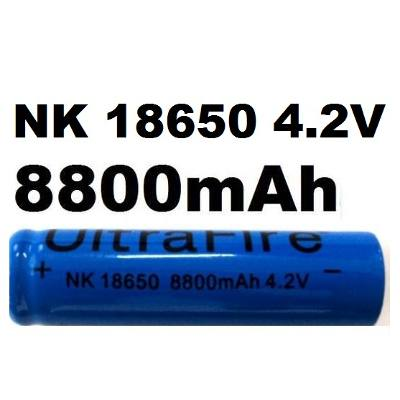
\includegraphics[scale=0.7]{figuras/bateria.jpg}
			\caption{Bateria NK 18650 Ultrafire.}
			\label{img:bateria}
		\end{figure}

		O Li-ion tem melhor relação de peso e potência que as baterias de Ni-MH ou Ni-Cd, tendo apenas o problema da tensão ser mais elevada.

		Usando o princípio da associação de fontes de tensão, resultará em um somatório das tensões das fontes. Quando 3 baterias de 4.2V são associadas em série temos o equivalente a um bateria de 12.6V, internamente em uma bateria é possível distinguir 3 células de 4.2V. Mas é preciso atentar que para resultar neste somatório todas as células ou fontes tem de estar com as polaridades sempre entre positivo para negativo ou vice versa.

	\subsubsection{Consumo energético}

		Foi realizada uma relação de consumo e capacidade de energia dos componentes para a escolha da bateria ideal, onde os motores consomem a maior parte da corrente.

		\begin{table}[H]
		\centering
		\caption{Consumo energético.}
		\label{tab:consumo_energético}
		\begin{tabular}{lllll}
		Componente               & Quantidade & Corrente unitária (mA) & Corrente total (mA) & Tensão (V) \\ \hline
		Ponte H                & 1          & 36                     & 36                  & 6          \\ \hline
		AtMega                 & 1          & 500                    & 500                 & 5          \\ \hline
		Motor DC               & 3          & 470                    & 1410                & 6          \\ \hline
		Módulo ESP8266         & 1          & 1000                   & 1000                & 3.3        \\ \hline
		Motor DC \\ 12V Aspiração & 1           & 4400                   & 4400                & 12         \\ \hline
		TOTAL                  &            &                        & 7421                & \\ \hline          
		\end{tabular}
		\end{table}

		De acordo com a tabela \ref{tab:consumo_energético}, é possível analisar a corrente e tensão de cada componente utilizado no projeto. Os componentes utilizados trabalharão com uma média de 7Ah, sendo que, um dos requisitos do robô é ter de aspirar um cômodo de maneira autônoma durante 30 minutos, com isto a corrente diminui para 3.5Ah.


	% subsection bateria (end)

	\subsection{Carregador} % (fold)
	\label{sub:carregador}
	
		Uma das grandes dificuldades na aplicação do sistema de alimentação em um projeto de eletrônico portátil é a forma com que se vai fornecer os ciclos de carga ao aparelho. No que tange as especificidades do nosso projeto, por ser um aspirador de pó que opera de forma autônoma, o maior desafio foi encontrar uma maneira de fazer com que o robô, após notar a necessidade, se dirigisse a sua base e começasse a se recarregar da forma mais simples e prática possível. 

Depois de diversas pesquisas e muitas hipóteses consideradas, chegou-se em consenso de que o princípio de carregamento por indução eletromagnética é o que mais se adequa ao nosso caso, já que não é necessário a conexão de cabos/conectores.

A indução eletromagnética consiste basicamente no surgimento de uma corrente elétrica oriunda de um fluxo magnético próximo de um condutor. O conceito é antigo e teve o princípio do raciocínio em 1820, quando Hans Christian Oesterd descobriu que cargas elétricas em movimento davam origem a um campo magnético.

 Tal descoberta levou diversos estudiosos da época a creer que o inverso também deveria ser possível de acontecer, ou seja: a varição do campo magnético levaria a uma produção de corrente elétrica. Michael Faraday, também dinamarquês, em 1931, batizou esse comportamento como indução eletromagnética e comprovou tal teoria através daquela que é conhecida até hoje com a Lei de Faraday.

 \begin{figure}[H]
	\centering
	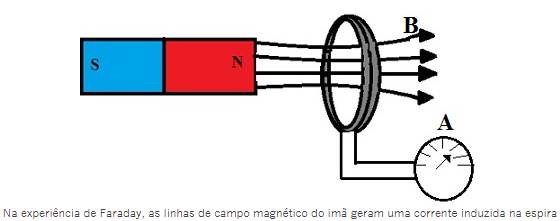
\includegraphics[scale=0.7]{figuras/carregador_inducao}
	\caption{Experiência de Faraday.}
	\label{img:faraday}
\end{figure}

A Lei de Faraday diz que uma força eletromotriz é produzida por condutores elétricos que se movimentam num campo magnético uniforme, ou então por um campo magnético variável. Tem uma melhor exemplificação da seguinte forma:


	$Fem = \frac{-d \phi }{dt}$


Sendo Fem a força eletromotriz (V), $\phi$ o fluxo magnético e t o tempo. Algum tempo depois James Clerk Maxwell, analisando o experimento de Faraday, escreveu uma outra lei que relaciona os campos elétrico e magnético, como podemos ver abaixo:


	$\nabla xE = \frac{-dB}{dt}$


Sendo $\nabla$ o operador nabla, E o campo elétrico e B o campo magnético. Analisando essa formulação conclui-se que o rotacional do campo elétrico é igual ao oposto da variação do campo magnético no tempo.


Esse conceito já é frequentemente utilizado em transformadores elétricos, motores, máquinas de indução em geral que hoje também englobam os carregadores mais modernos, afim de fornecer correntes de carga para baterias, especialmente para aparelhos como notebooks, tablets, smartphones e  e etc.

 \begin{figure}[H]
	\centering
	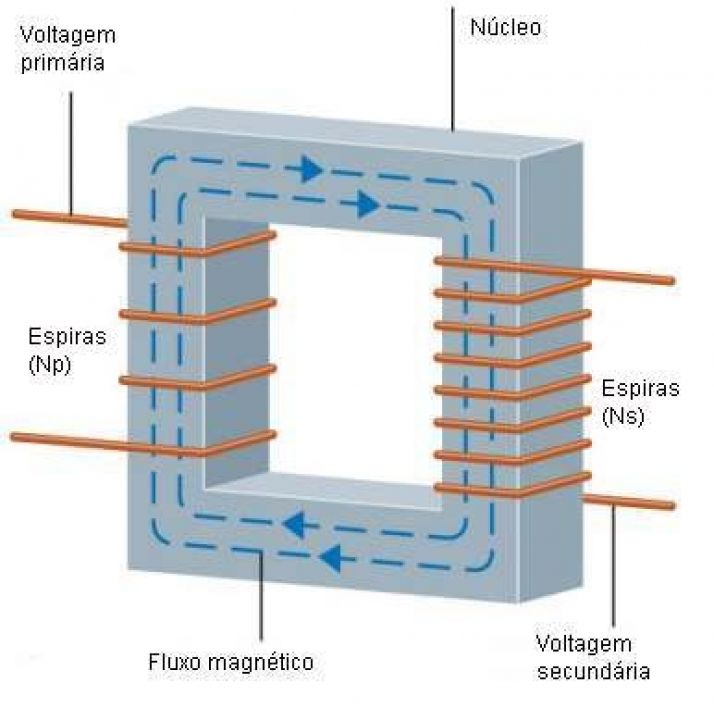
\includegraphics[scale=0.5]{figuras/transformador}
	\caption{Transformador elétrico.}
	\label{img:transformador}
\end{figure}

 \begin{figure}[H]
	\centering
	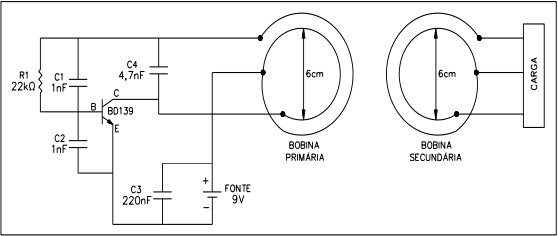
\includegraphics[scale=0.5]{figuras/diagrama_eletrico}
	\caption{Diagrama elétrico.}
	\label{img:diagrama_eletrico}
\end{figure}

Tendo como base experimentos já realizados que visaram a construção de um carregador por indução eletromagnética de forma artezanal, o grupo decidiu que deveríamos agir com a mesma linha de pensamento afim de ter o carregador para o projeto.

A construção demandou o uso de 3 capacitores, 1 resistor, 1 transistor, vários indutores (bobinas) e uma fonte de tensão contínua afim de se obter um circuito semelhante ao demonstrado na última figura.


	% subsection carregador (end)
% section alimentação (end)

\section{Navegação} % (fold)
\label{sec:navegação2}
	
	Como o processamento de todas as informações obtidas durante a navegação ocorrerá na base, sabe-se que o tempo de resposta do servidor é uma variável importante quando se refere a um sistema de tempo real, como o proposto pelo projeto. Dessa maneira, fez-se necessária a implantação do \textit{patch} \textit{rt\_preempt} no kernel do linux presente na \textit{raspberry}. Para isso, utilizamos como fonte de conhecimento a wiki oficial do projeto \textit{RT\_preempt}, disponível \href{https://rt.wiki.kernel.org/index.php/Main_Page}{aqui}.

	Com a configuração e recompilação do kernel com este \textit{patch}, obtivemos um tempo de resposta aproximado de 19 micro segundos, o que foi considerado bom pela equipe do projeto. Uma análise foi feita utilizando o \textit{script} \textit{cylicltest}, da mesma equipe \textit{RT\_preempt}, para calcular o tempo mínimo, médio e máximo de resposta. Na simulação foi utilizado um processo com prioridade 80, com 100.000 (cem mil) \textit{loops} a um intervalo de 500 micro segundos, obtendo o resultado apresentado na Figura \ref{img:tempo_de_resposta}.

	\begin{figure}[H]
		\centering
		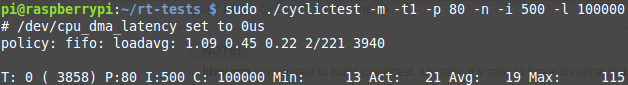
\includegraphics[scale=0.7]{figuras/tempo_de_resposta.png}
		\caption{Tempo de resposta do servidor.}
		\label{img:tempo_de_resposta}
	\end{figure}

% section navegação (end)


\section{Estrutura do Robô} % (fold)
\label{sec:estrutura_do_robô}

Nesta seção pode-se visualizar os processos que levaram a construção da base do robô, componente responsável pela locomoção e a integração de todos os componentes. E as soluções que foram tomadas para a melhoria da construção baseadas em testes feitos com a estrutura.

\subsection{Fabricação}

Ocorreram, durante o processo de fabricação da estrutura, mudanças relacionadas ao material empregado na construção da base. A princípio, seria utilizado uma chapa de alumínio, porém foi verificado que a chapa de alumínio, além de possuir algumas dificuldades para serem usinadas e soldadas, deveria possuir uma espessura um pouco maior para não vibrar muito com a ação do sistema de sucção. Uma chapa de metal, mesmo sendo de alumínio, de 2 cm é extremamente pesada, o que se tornaria um problema para os sistemas de navegação e locomoção do robô. Por esse motivo, o alumínio foi substituído por uma chapa de aço de 2mm de espessura. A base construída possui 39 cm de diâmetro e uma área útil de 1100 cm$^2$, espaço suficiente para alocar todos os componentes do robô.

\begin{figure}[H]
	\centering
	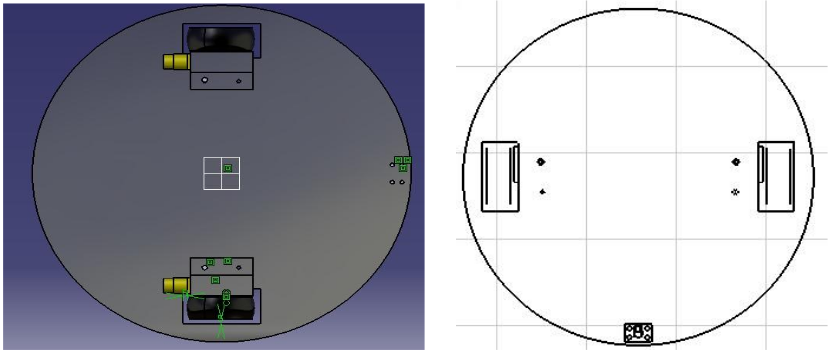
\includegraphics[scale=0.4]{figuras/vista_superior.png}
	\caption{Vista superior. A esquerda em 3D e a direita desenho técnico.}
	\label{img:vista_superior}
\end{figure}

O primeiro passo do processo de fabricação da estrutura foi a construção de um molde com as exatas dimensões da base, feito em madeira. Esse molde foi usado para verificar se o diâmetro de 39 cm seria suficiente para todos os componentes do robô e como seria feita a locação de cada componente, visando evitar erros no uso do material definitivo. Estando seguros do tamanho escolhido, foi feito o desenho circular em uma chapa de aço retangular utilizando um tipo de compasso, feito de prego e um lápis amarrado a uma linha de 20 cm. Em seguida, o corte circular foi feito com uma lixadeira. O diâmetro final da peça foi de 39 cm por causa da espessura da ferramenta que foi usada para o corte.

\begin{figure}[H]
	\centering
	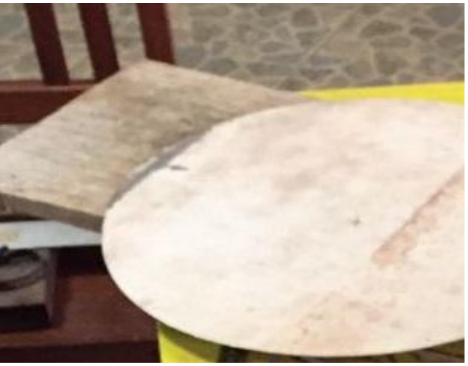
\includegraphics[scale=0.7]{figuras/primeiro_corte.png}
	\caption{Primeiro corte realizado para confecção da base.}
	\label{img:primeiro_corte}
\end{figure}

Com a base circular já pronta, foram feitas as marcações para os novos cortes e parafusos que entraram na estrutura, tudo isso, utilizando réguas e esquadros para se obter o melhor paralelismo possível para a peça final. Os cortes para o encaixe das rodas, foram feitos em formato retangular e exatamente do meio da peça. Para isso foi utilizado uma serra Tico Tico.

\begin{figure}[H]
	\centering
	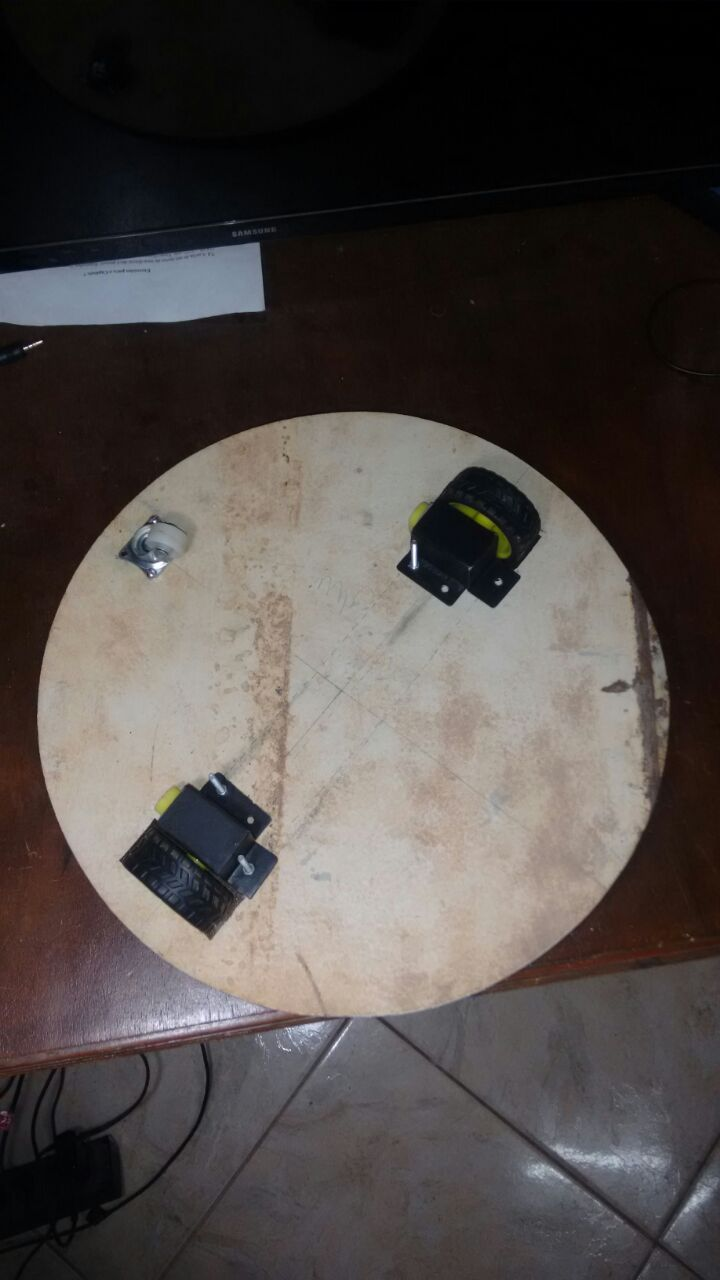
\includegraphics[scale=0.3]{figuras/serra_tico_tico.png}
	\caption{Base com as rodas montadas.}
	\label{img:serra_tico_tico}
\end{figure}

Tendo finalizado a estrutura principal da base, foi desenvolvido um suporte para fixar as rodas. Foram fabricados de tubo de aço retangular, “metalon”, de 30x25mm chapa 18. 

\begin{figure}[H]
	\centering
	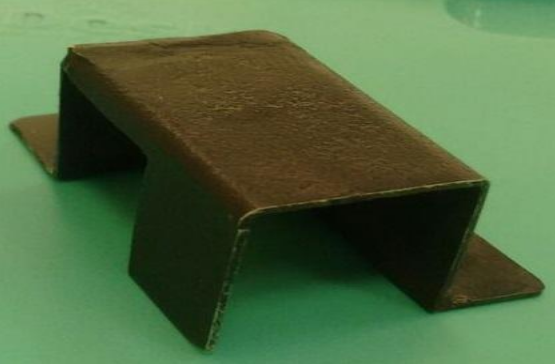
\includegraphics[scale=0.3]{figuras/suporte_fixar_rodas.png}
	\caption{Os suportes feitos para fixar as rodas.}
	\label{img:suporte_fixar_rodas}
\end{figure}

Com todos os componentes já produzidos, foram realizadas as furações na chapa com uma broca de 4mm para todos os parafusos e por fim os componentes foram montados e testados sua resistência e a capacidade de locomoção desse sistema. 

\begin{figure}[H]
	\centering
	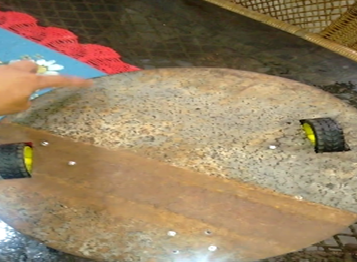
\includegraphics[scale=0.3]{figuras/base_teste.png}
	\caption{Teste 1 para verificar a estabilidade do carrinho.}
	\label{img:base_teste}
\end{figure}

Com o carrinho em movimento, a parte da estrutura que não possui roda livre era empurrada para baixo e se verificava o comportamento. Em todos os momentos o sistema voltava ao normal indicando que o uso de três rodas é viável dependendo da disposição dos componentes.

\begin{figure}[H]
	\centering
	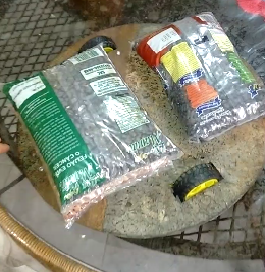
\includegraphics[scale=0.3]{figuras/base_teste_peso.png}
	\caption{Teste 2 – Verificando a resistência da estrutura.}
	\label{img:base_teste_peso}
\end{figure}

O teste consistia em colocar peso em cima da estrutura, aproximadamente 2 kg, e se empurrou o carrinho para ver seu comportamento.

\section{Documentação em CAD}

Durante o processo de fabricação da estrutura ocorreram alguns retrabalhos na documentação feita no CATIA, alguns sketches feitos eram mais complicados de serem usinados e poderiam nos trazer diversos erros de paralelismo na estrutura. Os desenhos finais da estrutura da base do motor são apresnetados a seguir.

\begin{figure}[H]
	\centering
	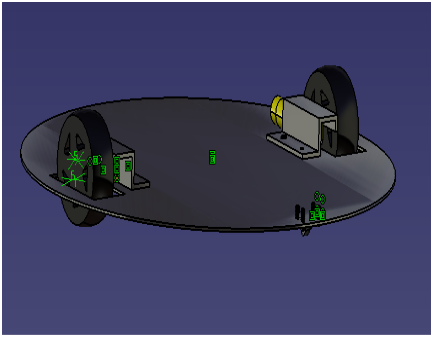
\includegraphics[scale=0.3]{figuras/vista_isometrica.png}
	\caption{Vista isométrica.}
	\label{img:vista_isometrica}
\end{figure}

\begin{figure}[H]
	\centering
	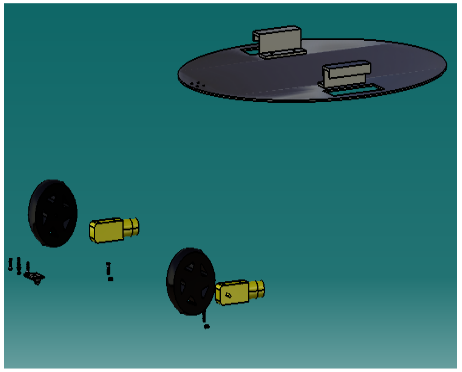
\includegraphics[scale=0.3]{figuras/vista_explodida.png}
	\caption{Vista explodida dos componentes.}
	\label{img:vista_explodida}
\end{figure}

\begin{figure}[H]
	\centering
	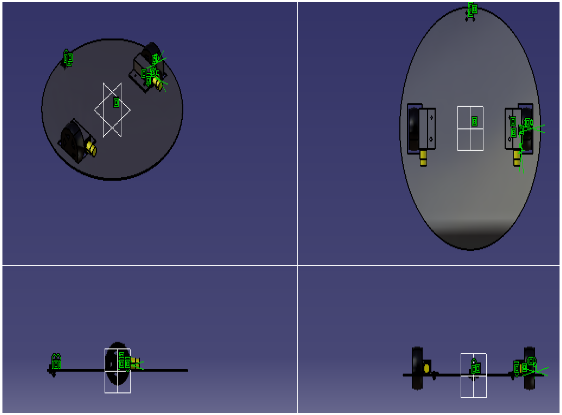
\includegraphics[scale=0.3]{figuras/vistas_em_corte.png}
	\caption{Vistas em corte.}
	\label{img:vistas_em_corte}
\end{figure}
% section estrutura_do_robô (end)

\subsection{Validação experimental} % (fold)
	\label{sub:validação_experimental}

	APRESENTAR AQUI OS TESTES PARA VALIDAÇÃO.

% \section{Estrutura da Base}

Nesta seção será avaliada a base de recarga do robô, que deve ser fabricada de acordo com as características da estrutura que integra todos os sistemas.

\subsection{Documentação em CAD}
Com a escolha de um carregamento através de indução, problemas com a usinagem dos encaixes entre o robô e seu sistema de carregamentos são solucionados. No sistema que será usado, a tolerância dimensional na fabricação se resume aos pneus do robô tendo um encaixe suave no trilho que serve de guia.

\begin{figure}[H]
	\centering
	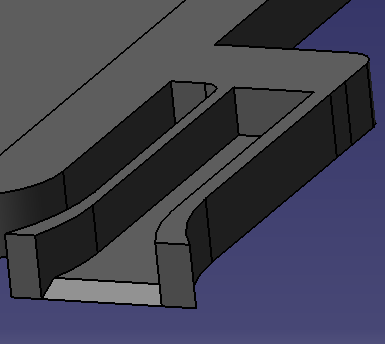
\includegraphics[scale=0.7]{figuras/trilho_base.png}
	\caption{Trilho que será como guia para as rodas.}
	\label{img:trilho_base}
\end{figure}

A ideia é que o robô seja guiado por esses trilhos e fique acomodado em cima da base de recarga. Além disso ao final do trilho fica a exata posição em que o sistema de recarga fica mais próximo dos conectores da bateria do robô, já que a proximidade entre os dois é fator muito importante para o tempo de recarga do robô.

\begin{figure}[H]
	\centering
	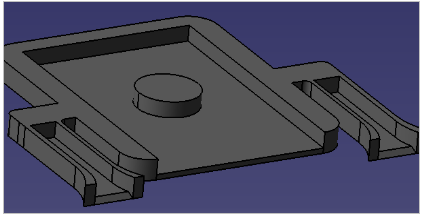
\includegraphics[scale=0.7]{figuras/desenho_base_recarga.png}
	\caption{Desenho da base de recarga.}
	\label{img:desenho_base_recarga}
\end{figure}


\section{Alimentação} % (fold)
\label{sec:alimentação}
	
	O sistema de alimentação pode ser dividido em 2 grandes grupos: \textit{Bateria} e \textit{Carregador}, os quais estão descritos nas sub-seções dispostas a seguir.

	\subsection{Bateria de íon-lítio (Li-Ion)} % (fold)
	\label{sub:bateria}
		
		De todos os tipos de baterias esta é, sem dúvida, a melhor. Suas vantagens são diversas e variadas e não é justamente por isso que elas são empregadas em larga escala nos novos eletrônicos.

		Não-tóxicas, com capacidade de carga duas vezes maior que as de Ni-MH e três vezes maior que as de NiCd, sem efeito memória (ou seja, a bateria não vai “viciar”) e também mais leves, afinal o lítio é um dos metais mais leves já conhecidos. A densidade do lítio também permite a criação de baterias com maior capacidade.

		Outro ponto que dá muito mais vantagens às baterias de Li-Ion é o fato de estas baterias dispensarem ciclos completos de cargas, ou seja, não é necessário esperar a carga acabar para carregá-la novamente e quando carrega não precisa esperar que ela seja preenchida por completo. Além disso, ao estar carregada por completo a bateria cessa automaticamente o recebimento de energia para evitar sobrecargas.

		Estas baterias, porém, demandam um cuidado maior por parte de seus usuários, como por exemplo, a não exposição a altas temperaturas que podem causar danos definitivos e até mesmo sua explosão.

	\subsubsection{Bateria utilizada}

		A 18650 é uma bateria de 4.2V e possui 8.8Ah. É de Li-íon assim como as baterias de celular, no entanto possuindo maior capacidade energética. A figura \ref{img:bateria} mostra a bateria NK 18650.

		\begin{figure}[H]
			\centering
			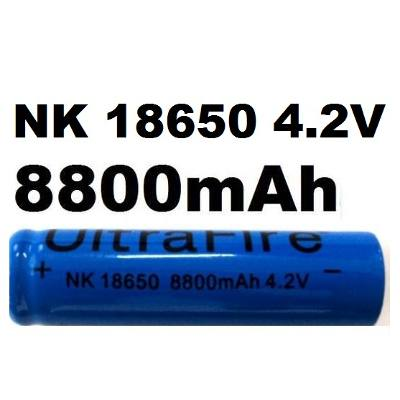
\includegraphics[scale=0.7]{figuras/bateria.jpg}
			\caption{Bateria NK 18650 Ultrafire.}
			\label{img:bateria}
		\end{figure}

		O Li-ion tem melhor relação de peso e potência que as baterias de Ni-MH ou Ni-Cd, tendo apenas o problema da tensão ser mais elevada.

		Usando o princípio da associação de fontes de tensão, resultará em um somatório das tensões das fontes. Quando 3 baterias de 4.2V são associadas em série temos o equivalente a um bateria de 12.6V, internamente em uma bateria é possível distinguir 3 células de 4.2V. Mas é preciso atentar que para resultar neste somatório todas as células ou fontes tem de estar com as polaridades sempre entre positivo para negativo ou vice versa.

	\subsubsection{Consumo energético}

		Foi realizada uma relação de consumo e capacidade de energia dos componentes para a escolha da bateria ideal, onde os motores consomem a maior parte da corrente.

		\begin{table}[H]
		\centering
		\caption{Consumo energético.}
		\label{tab:consumo_energético}
		\begin{tabular}{lllll}
		Componente               & Quantidade & Corrente unitária (mA) & Corrente total (mA) & Tensão (V) \\ \hline
		Ponte H                & 1          & 36                     & 36                  & 6          \\ \hline
		AtMega                 & 1          & 500                    & 500                 & 5          \\ \hline
		Motor DC               & 3          & 470                    & 1410                & 6          \\ \hline
		Módulo ESP8266         & 1          & 1000                   & 1000                & 3.3        \\ \hline
		Motor DC \\ 12V Aspiração & 1           & 4400                   & 4400                & 12         \\ \hline
		TOTAL                  &            &                        & 7421                & \\ \hline          
		\end{tabular}
		\end{table}

		De acordo com a tabela \ref{tab:consumo_energético}, é possível analisar a corrente e tensão de cada componente utilizado no projeto. Os componentes utilizados trabalharão com uma média de 7Ah, sendo que, um dos requisitos do robô é ter de aspirar um cômodo de maneira autônoma durante 30 minutos, com isto a corrente diminui para 3.5Ah.


	% subsection bateria (end)

	\subsection{Carregador} % (fold)
	\label{sub:carregador}
	
		Uma das grandes dificuldades na aplicação do sistema de alimentação em um projeto de eletrônico portátil é a forma com que se vai fornecer os ciclos de carga ao aparelho. No que tange as especificidades do nosso projeto, por ser um aspirador de pó que opera de forma autônoma, o maior desafio foi encontrar uma maneira de fazer com que o robô, após notar a necessidade, se dirigisse a sua base e começasse a se recarregar da forma mais simples e prática possível. 

Depois de diversas pesquisas e muitas hipóteses consideradas, chegou-se em consenso de que o princípio de carregamento por indução eletromagnética é o que mais se adequa ao nosso caso, já que não é necessário a conexão de cabos/conectores.

A indução eletromagnética consiste basicamente no surgimento de uma corrente elétrica oriunda de um fluxo magnético próximo de um condutor. O conceito é antigo e teve o princípio do raciocínio em 1820, quando Hans Christian Oesterd descobriu que cargas elétricas em movimento davam origem a um campo magnético.

 Tal descoberta levou diversos estudiosos da época a creer que o inverso também deveria ser possível de acontecer, ou seja: a varição do campo magnético levaria a uma produção de corrente elétrica. Michael Faraday, também dinamarquês, em 1931, batizou esse comportamento como indução eletromagnética e comprovou tal teoria através daquela que é conhecida até hoje com a Lei de Faraday.

 \begin{figure}[H]
	\centering
	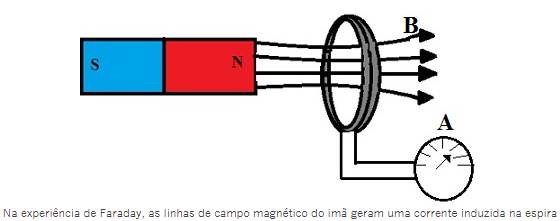
\includegraphics[scale=0.7]{figuras/carregador_inducao}
	\caption{Experiência de Faraday.}
	\label{img:faraday}
\end{figure}

A Lei de Faraday diz que uma força eletromotriz é produzida por condutores elétricos que se movimentam num campo magnético uniforme, ou então por um campo magnético variável. Tem uma melhor exemplificação da seguinte forma:


	$Fem = \frac{-d \phi }{dt}$


Sendo Fem a força eletromotriz (V), $\phi$ o fluxo magnético e t o tempo. Algum tempo depois James Clerk Maxwell, analisando o experimento de Faraday, escreveu uma outra lei que relaciona os campos elétrico e magnético, como podemos ver abaixo:


	$\nabla xE = \frac{-dB}{dt}$


Sendo $\nabla$ o operador nabla, E o campo elétrico e B o campo magnético. Analisando essa formulação conclui-se que o rotacional do campo elétrico é igual ao oposto da variação do campo magnético no tempo.


Esse conceito já é frequentemente utilizado em transformadores elétricos, motores, máquinas de indução em geral que hoje também englobam os carregadores mais modernos, afim de fornecer correntes de carga para baterias, especialmente para aparelhos como notebooks, tablets, smartphones e  e etc.

 \begin{figure}[H]
	\centering
	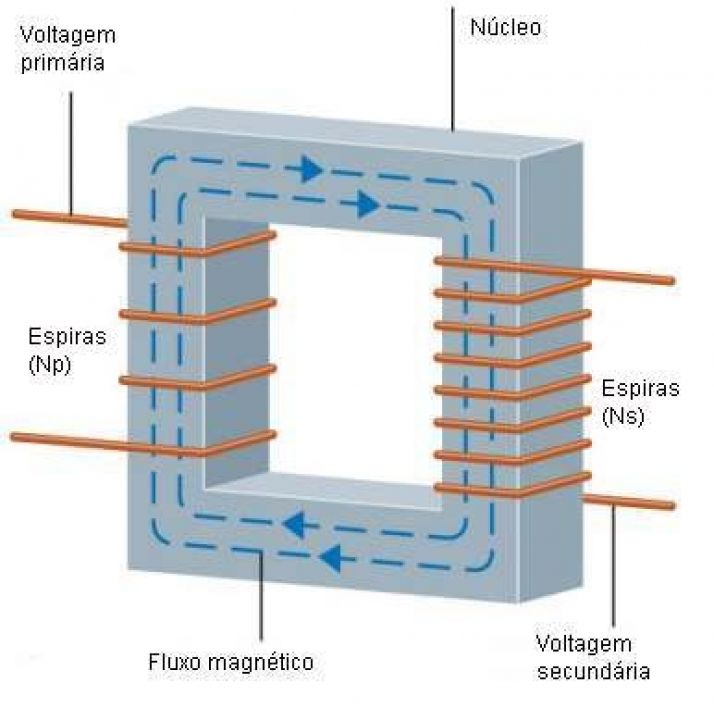
\includegraphics[scale=0.5]{figuras/transformador}
	\caption{Transformador elétrico.}
	\label{img:transformador}
\end{figure}

 \begin{figure}[H]
	\centering
	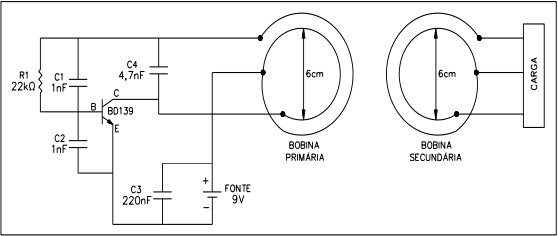
\includegraphics[scale=0.5]{figuras/diagrama_eletrico}
	\caption{Diagrama elétrico.}
	\label{img:diagrama_eletrico}
\end{figure}

Tendo como base experimentos já realizados que visaram a construção de um carregador por indução eletromagnética de forma artezanal, o grupo decidiu que deveríamos agir com a mesma linha de pensamento afim de ter o carregador para o projeto.

A construção demandou o uso de 3 capacitores, 1 resistor, 1 transistor, vários indutores (bobinas) e uma fonte de tensão contínua afim de se obter um circuito semelhante ao demonstrado na última figura.


	% subsection carregador (end)
% section alimentação (end)

\section{Estrutura da Base}

Nesta seção será avaliada a base de recarga do robô, que deve ser fabricada de acordo com as características da estrutura que integra todos os sistemas.

\subsection{Documentação em CAD}
Com a escolha de um carregamento através de indução, problemas com a usinagem dos encaixes entre o robô e seu sistema de carregamentos são solucionados. No sistema que será usado, a tolerância dimensional na fabricação se resume aos pneus do robô tendo um encaixe suave no trilho que serve de guia.

\begin{figure}[H]
	\centering
	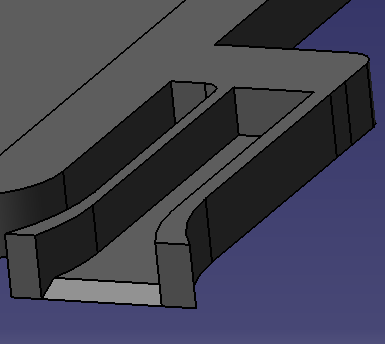
\includegraphics[scale=0.7]{figuras/trilho_base.png}
	\caption{Trilho que será como guia para as rodas.}
	\label{img:trilho_base}
\end{figure}

A ideia é que o robô seja guiado por esses trilhos e fique acomodado em cima da base de recarga. Além disso ao final do trilho fica a exata posição em que o sistema de recarga fica mais próximo dos conectores da bateria do robô, já que a proximidade entre os dois é fator muito importante para o tempo de recarga do robô.

\begin{figure}[H]
	\centering
	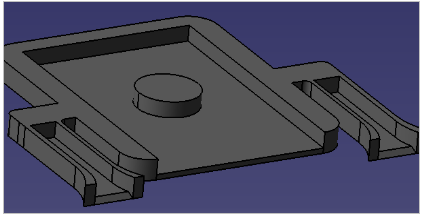
\includegraphics[scale=0.7]{figuras/desenho_base_recarga.png}
	\caption{Desenho da base de recarga.}
	\label{img:desenho_base_recarga}
\end{figure}


\section{Sucção} % (fold)
\label{sec:sucção2}
	Essa sessão visa documentar o método de construção do sistema de sucção do robô, descrevendo a construção dos protótipos e as decisões tomadas com base em testes realizados em cada protótipo. 

	\subsection{Metodologia de construção}
	\label{sub:metodologia_de_construção}
		Para a execução do projeto proposto foram adquiridos três coolers comerciais de 14 cm com as especificações apresentadas na tabela \ref{tab:especificações_coolers}.

		\begin{table}[H]
			\centering
			\caption{Dados do cooler}
			\label{tab:especificações_coolers}
			\begin{tabular}{ll}
				Potencia                                              & 1.44 W               \\
				Voltagem                                              & 12 V                 \\
				Velocidade                                            & 1200+-10\% RPM       \\
			\begin{tabular}[c]{@{}l@{}}Fluxo de ar\end{tabular} & 1.36 $m^3$/min (48 CFM)
			\end{tabular}
		\end{table}

		O projeto baseava-se em apenas dois coolers, mas foram adquiridos três caso o resultado com dois não retornasse uma boa sucção. A montagem consiste em os cooler ligados lado a lado dentro de uma caixa hermeticamente fechada. Utilizando os três coolers, foram feitos os primeiros testes para medir a eficiência dessa montagem. Foi feito um furo de pequeno diâmetro na parte oposta à dos coolers, por onde deve entrar o ar.

		\begin{figure}[H]
			\centering
			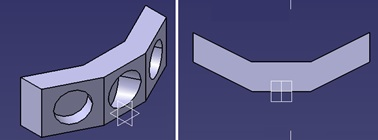
\includegraphics[scale=1]{figuras/asppc2_1.jpg}
			\caption{Vista isométrica e superior da montagem, onde os buracos representam a posição dos coolers.}
			\label{img:vista_isometrica_de_montagem}
		\end{figure}

		Os coolers foram ligados à voltagem de 12V com corrente de 1.5 A, mas o resultado não foi satisfatório, pois não houve nenhuma sucção mesmo alterando o diâmetro do buraco e sua posição. Foi suposto que o problema seriam os coolers, então foi planejada uma montagem com um deles para verificar seu funcionamento isolado.

		Foi realizado um teste simples, utilizando um cooler menor de 5 cm para verificar o funcionamento do modelo de construção. A figura \ref{img:cooler_5cm} mostra o sistema construído.

		\begin{figure}[H]
			\centering
			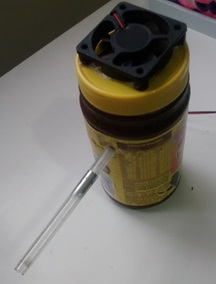
\includegraphics[scale=1]{figuras/asppc2_2.jpg}
			\caption{Montagem com cooler de 5 cm.}
			\label{img:cooler_5cm}
		\end{figure}

		O sistema foi ligado na fonte e este protótipo apresentou resultados positivos, apesar da sucção fraca por conta da voltagem e corrente do cooler serem baixos. O mesmo modelo foi construído em maior escala para utilizar o cooler maior. A figura \ref{img:cooler_14cm} mostra outro modelo construído.

		\begin{figure}[H]
			\centering
			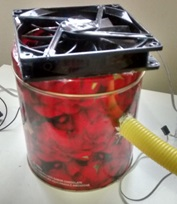
\includegraphics[scale=1]{figuras/asppc2_3.jpg}
			\caption{Montagem com cooler de 14 cm.}
			\label{img:cooler_14cm}
		\end{figure}

		Foi fornecido a tensão de 12V e corrente de 1.5 A ao sistema, mas apresentou-se uma eficiência muito baixa, com sucção quase imperceptível. Então, utilizando uma fonte de tensão, foi-se elevando a tensão até que ele indicasse uma melhora. Foi observado que enquanto a tensão era modificando, as hélices passavam a girar com maior velocidade passando a sugar com maior força. Ao fornecer o valor de tensão de 30 V, foi que o sistema alcançou um resultado que seria ótimo para o projeto. Mas seria inviável a fabricação do robô com uma bateria que fornecesse tal tensão. 

		O último teste utilizando estes coolers, consistiu em aumentar a potência do sistema construindo-o com dois coolers utilizando o mesmo esquema de construção, visando uma alimentação de menor tensão para os motores. Foi reduzida a altura do sistema, a fim de reduzir perdas de carga, e adicionado um cooler em uma das paredes, ao final obteve o protótipo mostrado na figura \ref{img:coolers_14cm}.

		\begin{figure}[H]
			\centering
			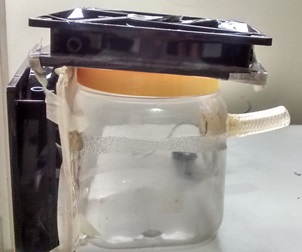
\includegraphics[scale=1]{figuras/asppc2_4.jpg}
			\caption{Protótipo com dois coolers de 14 cm.}
			\label{img:coolers_14cm}
		\end{figure}

		Era esperado que com essa nova montagem, a eficiência fosse aumentada ao dobrar a potência do sistema, mas o resultado foi negativo, pois não apresentou mudanças com relação ao modelo com um cooler. Com os resultados obtidos com as montagens mostradas, o grupo chegou à conclusão de que os coolers não seriam utilizados, pois não mostraram resultados bons que fossem viáveis ao projeto. Os motores elétricos dos coolers possuíam uma potência incompatível com o tipo e o tamanho da hélice do mesmo, gerando um fluxo de massa baixo, menor que o indicado pelos fabricantes. 

		Diante dos problemas, foram feitas pesquisas a respeito de novos modelos de construção que fossem eficientes, apresentando uma sucção forte, dentro dos limites de tensão possíveis no projeto. As hélices são um tipo de “ventilador axial”, que força o ar a passar por elas, gerando um fluxo de ar segue transversal à direção do cooler. Existe também outro tipo de ventilador, conhecido como “ventilador centrífugo”, onde suas hélices são dispostas de forma diferente, como mostra a figura \ref{img:ventilador_centrífugo}.

		\begin{figure}[H]
			\centering
			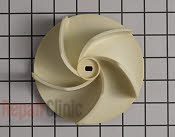
\includegraphics[scale=1]{figuras/asppc2_5.jpg}
			\caption{Hélices do ventilador centrífugo.}
			\label{img:ventilador_centrífugo}
		\end{figure}

		O “ventilador centrífugo” acelera o ar radialmente, fazendo com que a energia cinética da rotação das hélices aumente a pressão do ar, resultando em um fluxo de alta velocidade na saída. Foi escolhida essa hélice para a construção de novos protótipos.

		\begin{figure}[H]
			\centering
			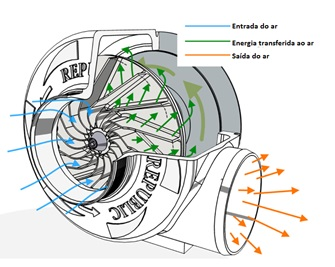
\includegraphics[scale=1]{figuras/asppc2_6.jpg}
			\caption{Fluxo de ar em um ventilador de ar centrífugo.\href{https://www.republic-mfg.com/blowers/republic-centrifugal-blower.asp}{Republic Manufacturing}}
			\label{img:ventilador_centrífugo}
		\end{figure}

		Para evitar o problema de falta de potência, foi escolhido um motor com maior potência e rotação nominal se comparado ao motor do cooler. Foi escolhido um motor DC 12V com as especificações apresentadas na tabela \ref{tab:motor_12V}.

		\begin{table}[H]
			\centering
			\caption{Dados do motor DC 12 Volts.}
			\label{tab:motor_12V}
			\begin{tabular}{ll}
				Potencia   & 40.55W          \\
				Voltagem   & 13.5 V          \\
				Velocidade & 28086+-10\% RPM \\
				Torque     & 55.19 mN.m     
			\end{tabular}
		\end{table}

		As hélices foram construídas em alumínio e grudadas em uma pequena base com furo para encaixar o eixo do motor (\ref{img:hélices_alumínio}).

		\begin{figure}[H]
			\centering
			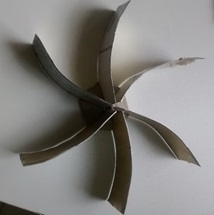
\includegraphics[scale=1]{figuras/asppc2_7.jpg}
			\caption{Hélices construídas em alumínio.}
			\label{img:hélices_alumínio}
		\end{figure}

		Utilizando CD’s, papelão, plástico em formato cilíndrico a estrutura final desse protótipo é mostrada na figura \ref{img:protótipo_CD}.  

		\begin{figure}[H]
			\centering
			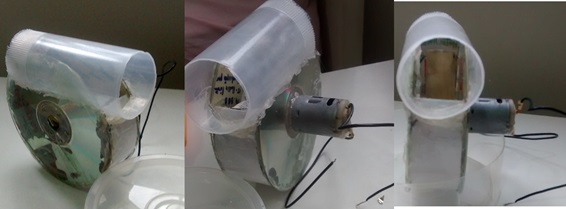
\includegraphics[scale=1]{figuras/asppc2_8.jpg}
			\caption{Vistas do protótipo feito com CD’s.}
			\label{img:protótipo_CD}
		\end{figure}

		Foi realizado o teste com o novo protótipo, mas por defeitos de fabricação, as hélices durante a rotação colidiam com a estrutura, assim o ar era soprado com menor velocidade, consequentemente sugava um fluxo baixo de ar. 

		Foi feita outro protótipo utilizando o mesmo modelo de hélice construída utilizando CD’s seguindo o mesmo modelo de estrutura, mas novamente, as hélices não giravam livremente, pois colidiam com as outras partes da estrutura. Graças à essas assimetrias e defeitos de fabricação foi observado uma grande vibração do sistema. Diante da dificuldade de construir uma estrutura sem defeitos e visando reduzir as vibrações, para que ela não danifique a estrutura do robô e aumentar a eficiência do ventilador foi adotada a solução de adquirir a hélice comercial, garantindo uma construção sem defeitos. O motor para movimentar a hélice é de 12V, potência de 52.8 W, corrente de 4.4 A.

		\begin{figure}[H]
			\centering
			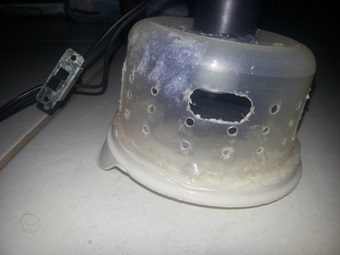
\includegraphics[scale=1]{figuras/asppc2_9.jpg}
			\caption{Motor de 52.8W instalado na estrutura de aspiração.}
			\label{img:estrutura_motor_52.8W}
		\end{figure}

		Foi realizada a montagem do protótipo utilizando a nova hélice. Foram utilizados dois compartimentos de plásticos, em um foi acoplado o conjunto hélice motor, e nas laterais foram feitos furos para a saída de ar. Foi colocada uma divisão entre os dois compartimentos com um filtro para a sujeira. Foi feito um furo no segundo compartimento para encaixar a mangueira a qual irá ser a ponta da sucção. Conectou-se as partes e foram feitos os testes ligando-a fonte de 12V e 4.4 A. O resultado foi positivo apresentando uma sucção forte, sugando toda a sujeira que foi disponibilizada para o teste.

		\begin{figure}[H]
			\centering
			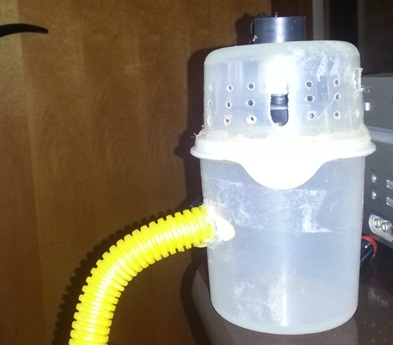
\includegraphics[scale=1]{figuras/asppc2_10.jpg}
			\caption{Sistema de sucção com o compartimento de sujeira.}
			\label{img:sistema_com_compartimento}
		\end{figure}

		Para aumentar a eficiência de limpeza, foi adicionado ao sistema de sucção uma vassoura mágica. A fricção dela com o solo faz com que a sujeira seja carregada para seu compartimento interno, mas para garantir uma boa limpeza ela deve passar pelo mesmo local várias vezes. Como o robô irá percorrer a trajetória em linha reta com velocidade constante sem realizar muitas passagens pelo mesmo local, foi acoplado um motor DC de 6V e 0.1 A no eixo da vassoura para garantir um aumento na eficiência na coleta da sujeira. Ao realizar o teste, observou-se que por conta da grande velocidade de rotação do motor, as partículas de sujeiras eram lançadas para longe, ao invés de serem carregadas para seu interior. Foi colocado um tecido com pelos atrás da vassoura, limitando o movimento de partículas naquela direção, garantindo que elas fossem depositadas no interior da vassoura mágica.

		\begin{figure}[H]
			\centering
			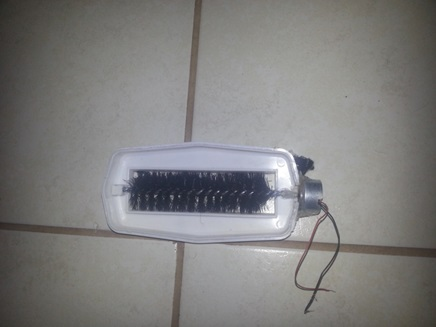
\includegraphics[scale=1]{figuras/asppc2_11.jpg}
			\caption{Escova mágica conectada ao motor DC de 6V.}
			\label{img:escova_com_motor}
		\end{figure}

		\begin{figure}[H]
			\centering
			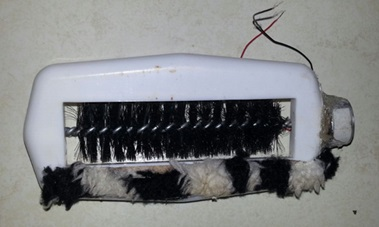
\includegraphics[scale=1]{figuras/asppc2_12.jpg}
			\caption{Parte inferior da escova mágica com o tecido de contenção das partículas.}
			\label{img:escova_com_tecido}
		\end{figure}

		Com os dois subsistemas de limpeza prontos e funcionando, foi feita a conexão entre eles por uma mangueira sanfonada, para que ela sugue as partículas de sujeiras que a vassoura colhe. Foi feito um furo na parte superior da estrutura da vassoura da forma da ponta de mangueira, que foi achatada para aumentar o comprimento de aspiração da sujeira que fica interna a vassoura mágica. O resultado do protótipo é mostrado na figura abaixo.

		\begin{figure}[H]
			\centering
			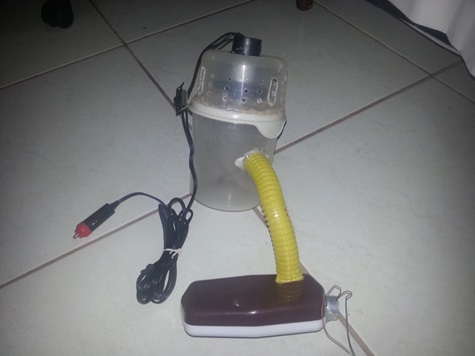
\includegraphics[scale=1]{figuras/asppc2_13.jpg}
			\caption{Subsistema de sucção completo.}
			\label{img:sistema_completo}
		\end{figure}

		Foi realizado o teste das duas peças integradas, simulou-se o movimento do robô passando-o apenas uma vez por cima da sujeira. O resultado foi positivo, o sistema foi capaz de colher cerca de 80\% das partículas que foram colocadas para teste.
	% subsection metodologia de construção (end)
% section sucção (end)

\section{Sensoriamento} % (fold)
\label{sec:sensoriamento2}

	Após definir as especificações dos componentes na sessão \ref{sec:sensoriamento}, será descrito a seguir de forma detalhada as estratégias seguidas pelo grupo para atender aos requisitos do projeto. Tambem serão apresentadas as simulações realizadas para validar os conceitos aplicados, resultados práticos serão apresentados em um momento posterior.

	A parte do projeto de eletrônica responsável pela comunicação será apresentada na sessão \ref{sub:hardware}.

	\subsection{Instrumentação} % (fold)
	\label{sub:instrumentação2}
		A instrumentação foi dividida em três subgrupos, cada um com um foco especifico para garantir a integridade do robô \textit{R2-PI2}, esses subgrupos são apresentados a seguir.

		\subsubsection{Controle de distância}
		\label{sub:Controle_de_distância}
		A estratégia de controle utilizada na locomoção do R2-PI2, analisa as seguintes situações, o robô se locomoverá sempre para a frente enquanto não encontrar obstáculos em seu caminho. Na detecção de um objeto, os sensores posicionados a direta e a esquerda do robô farão a medição de distância. O aspirador tomará a decisão de desviar para o lado contrário da menor distância medida ou na ausência da mesma. Na possibilidade de ausência de distância ou impossibilidade de cálculos, o desvio será feito a direita por padrão. A figura \ref{img:circuito_de_controle_dos_motores} mostra o fluxograma do algoritmo utilizado na locomoção do aspirador.

		\begin{figure}[H]
			\centering
			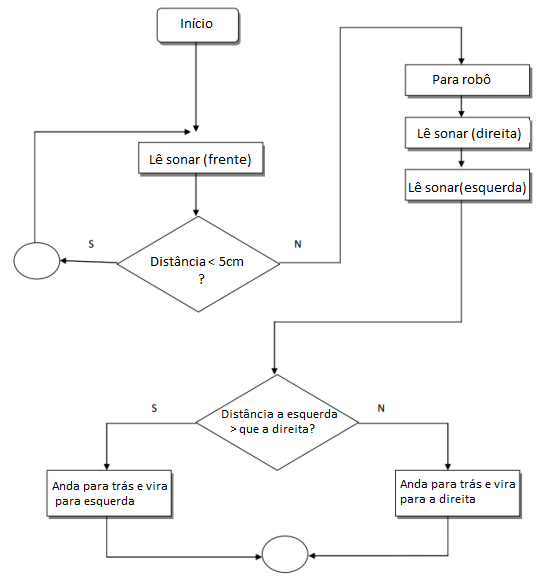
\includegraphics[scale=0.8]{figuras/fluxograma_eletronica.png}
			\caption{Fluxograma do algoritmo de locomoção do R2-PI2, realizado pela equipe de eletrônica para testes iniciais.}
			\label{img:circuito_de_controle_dos_motores}
		\end{figure}

		No caso da identificação de degraus ou desníveis o algoritmo consiste na simples análise de obstáculos ou não. Por limitação do sensor IR, a distância máxima medida é de 2.5 cm, então enquanto uma distância escolhida como aproximadamente 1cm estiver sendo medida, o que significa que o robô está em contato com o chão, ele continuará se movimentando normalmente, quando essa distância medida for maior que 1 cm, o aspirador irá parar, dar uma ré e escolher a melhor rota para continuar seguindo.

		Tanto no código de medição de distância com o ultrassom, quanto no com sensor IR utilizou-se a técnica de filtragem por médias móveis que consiste em fazer várias amostragens de um parâmetro e depois tirar a média das mesmas. O filtro ajudou bastante no problema de leituras oscilantes nos sensores. 

		\subsubsection{Monitoramento da bateria}
		\label{sub:Monitoramento_da_bateria}
		Com carga máxima, a bateria escolhida terá 12,6V e ela deixará de fornecer a corrente adequada ao circuito quando chegar a 8,25V (aproximadamente 66\% da bateria total). Para evitar que a bateria chegue a 8,25V no meio da execução da limpeza, um circuito comparador de tensão irá verificar continuamente qual a voltagem da bateria.

		Além de enviar o sinal para o microcontrolador, será feita uma interface visual com 5 LEDs que vão indicar quando a bateria está com carga total e quando a bateria está perto da carga mínima (8,25V), conforme a figura \ref{img:faixa_de_tensão}.

		\begin{figure}[H]
			\centering
			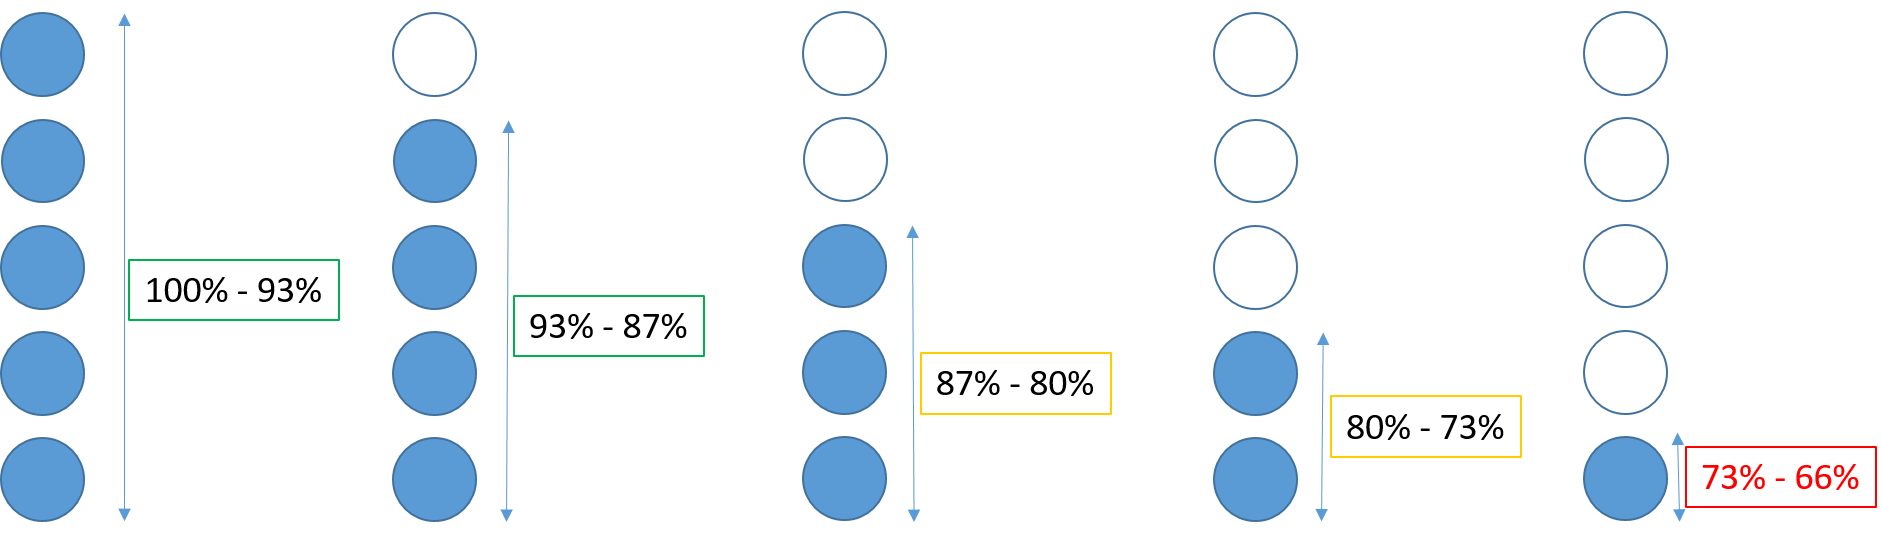
\includegraphics[scale=0.3]{figuras/LEDs.png}
			\caption{Aproximação das faixas de tensão apresentadas pelos LEDs.}
			\label{img:faixa_de_tensão}
		\end{figure}

		A queda de tensão será apresentada em cinco LEDs que foram divididos em faixas muito próximas de tensão útil. Conforme os seguintes cálculos:

		\begin{equation}
		\label{eq:equação_medidor_bateria}
			\frac{Tensão\ máxima - tensão\ mínima}{5}  
		\end{equation}

		Substituindo os valores em (\ref{eq:equação_medidor_bateria}), temos:

		\begin{equation}
		\label{eq:equação_medidor_bateria_2}
			\frac{100-66}{5} = 6,8  
		\end{equation}

		As faixas então foram definidas como:

		\begin{itemize}
			\item \textbf{Faixa 1}: 100\% $\sim$ 93,2\%
			\item \textbf{Faixa 2}: 93,2\% $\sim$ 86,4\%
			\item \textbf{Faixa 3}: 86,4\% $\sim$ 79,6\%
			\item \textbf{Faixa 4}: 79,6\% $\sim$ 72,8\%
			\item \textbf{Faixa 5}: 72,8\% $\sim$ 66\%
		\end{itemize}
		
		Considerando que o sistema de sucção consome cerca de seis vezes mais corrente do que o sistema de navegação do robô (4750mA - 836mA) e que são cinco faixas de tensão, estimou-se que um quinto da tensão útil é suficiente para o robô voltar para a base de carregamento com o sistema de sucção desligado. No entanto, sabendo que a curva de descarga de uma bateria não é linear, apenas após os testes empíricos será possível determinar com maior segurança se um ou dois quintos da tensão útil serão colocados à disposição do sistema de navegação para o robô poder retornar à base. 

		Assim, enquanto a tensão da bateria estiver dentro das quatro faixas de tensão, o robô estará executando a rotina de limpeza e quando estiver na última faixa ele estará retornando para a base. 

		As faixas de tensão foram projetadas a partir de um divisor de tensão com cinco saídas sendo que cada saída é o limite inferior da faixa.

		\begin{figure}[H]
			\centering
			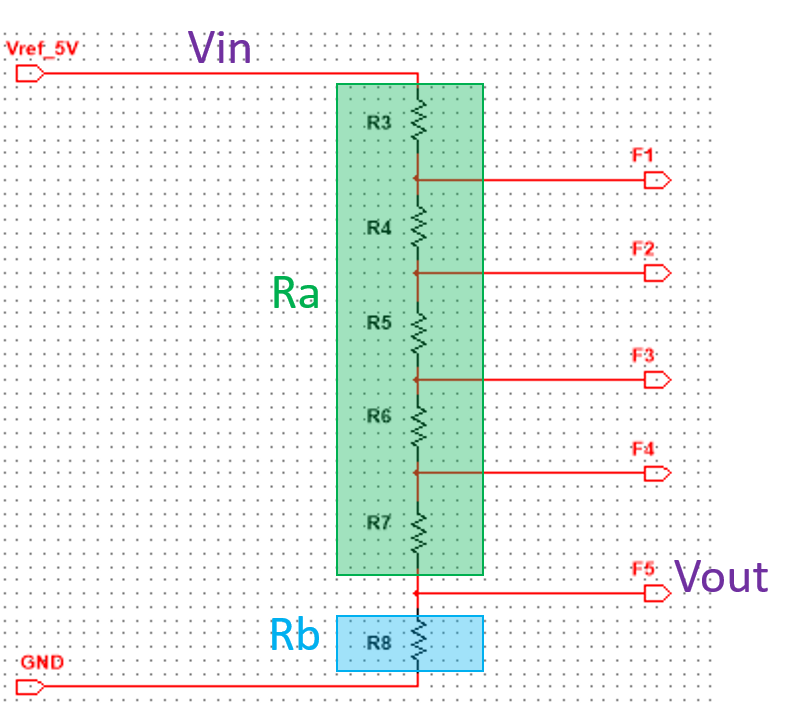
\includegraphics[scale=0.5]{figuras/Divisor1.png}
			\caption{Divisor de tensão.}
			\label{img:divisor_de_tensão}
		\end{figure}

		Fazendo o divisor de tensão com Ra e Rb, tem-se que:

		\begin{equation}
		\label{eq:divisor_de_tensão}
			Vout= \frac{Rb * Vin}{Ra + Rb} 
		\end{equation}

		Sabendo que ${Vout = 0,66 * Vin}$, substituimos \textit{Vout} na equação \ref{eq:divisor_de_tensão}:
		
		\begin{equation}
		\label{eq:divisor_de_tensão_2}
			0,66 *Vin=\frac{Rb *Vin}{Ra + Rb} 
		\end{equation}

		Que resulta em:

		\begin{equation}
		\label{eq:divisor_de_tensão_3}
			0,66 * Ra + 0,66 * Rb = Rb
		\end{equation}

		Se Rb=10K$\Omega$, substituimos na equação \ref{eq:divisor_de_tensão_3} e obtemos:

		\begin{equation}
		\label{eq:divisor_de_tensão_4}
			Ra=\frac{10K - 0,66 * 10K}{0,66} \simeq 5K
		\end{equation}

		Como as faixas devem ter a aproximadamente a mesma variação de tensão, os resistores R3, R4, R5, R6 e R7 devem ter o mesmo valor e sua associação em série deve ser igual a 5K$\Omega$ (Ra), assim os valores das resistências do divisor de tensão devem ser:

		\begin{equation}
		\label{eq:divisor_de_tensão_5}
			R3 + R4 + R5 + R6 + R7 = 5K\ =>\  
			R3 = R4 = R5 = R6 = R7 = 1K
		\end{equation}

		\begin{equation}
		\label{eq:divisor_de_tensão_6}
			Rb = Rc = 10K
		\end{equation}

		Para confirmar se o divisor proposto realmente cumpre os requisitos do projeto, foi realizada a simulação utilizando o software MultiSim do divisor aplicando uma tensão de 10V e o resultado obtido foi satisfatório.

		\begin{figure}[H]
			\centering
			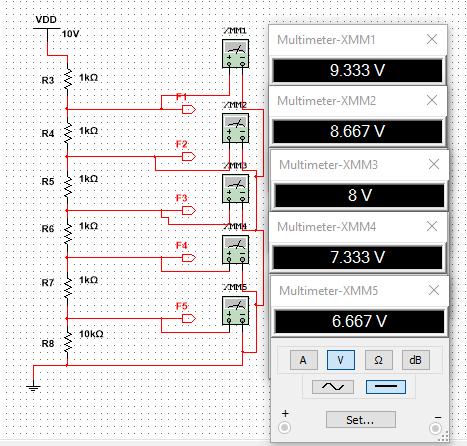
\includegraphics[scale=0.8]{figuras/Divisor1_simu.png}
			\caption{Simulação do divisor de tensão.}
			\label{img:divisor_de_tesnão_simulado}
		\end{figure}


		Para o circuito acima funcionar bem, a tensão de entrada do divisor de tensão deverá ser igual a tensão máxima da bateria. Como a tensão máxima da bateria é de 12.6V, fica inviável geral um sinal constante de 12.6V apenas para servir como referência do divisor. Sabendo que o ATMega gera um sinal de 5V, a tensão da bateria passará por um divisor de tensão  que será projetado para transformar os 12.6V em 5V de modo que seja possível utilizar os 5V do ATMega no medidor de bateria.

		Sabendo que a tensão de saída do novo resistor (Vout2) deve ser 5V e que a tensão de entrada (Vin2) é de 12.6V as resistências (Rc e Rd) utilizadas podem ser calculadas pela seguinte expressão:

		\begin{equation}
		\label{eq:divisor_de_tensão_7}
			Vout2 =\frac{Rc * Vin2}{Rc + Rd}
		\end{equation}

		Substituindo os valores em \ref{eq:divisor_de_tensão_7}, temos:

		\begin{equation}
		\label{eq:divisor_de_tensão_8}
			5\ =\frac{Rc * 12.6}{Rc + Rd}\ =>\ 7.6 * Rc = 5 *Rd
		\end{equation}

		Se Rc=1K$\Omega$, logo:

		\begin{equation}
		\label{eq:divisor_de_tensão_9}
			Rd =\frac{7.6}{5} \simeq 1.5K
		\end{equation}

		Para verificar o divisor projeto se adequa às necessidades do projeto, foi feita a simulação no software MultiSim e o resultado encontrado foi satisfatório. A variação de 0,04V corresponde a 0,3\% da tensão máxima e, portanto, não prejudicará o sistema de medição da bateria.

		\begin{figure}[H]
			\centering
			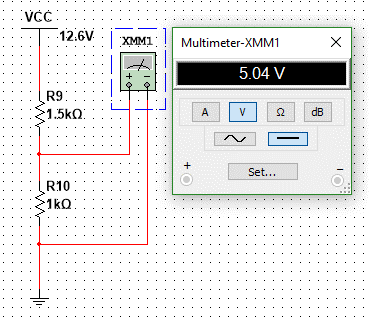
\includegraphics[scale=0.8]{figuras/Divisor2_simu.png}
			\caption{Simulação do divisor de tensão de 12.6V para 5V.}
			\label{img:divisor_de_tesnão_simulado}
		\end{figure}

		O circuito completo do medidor de bateria é apresentado na figura \ref{img:medidor_de_bateria}.

		\begin{figure}[H]
			\centering
			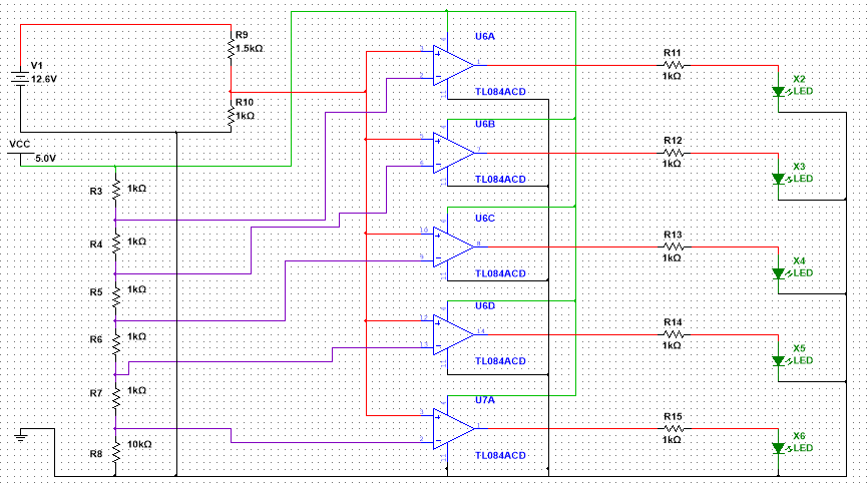
\includegraphics[scale=0.7]{figuras/Med_bateria.png}
			\caption{Circuito do medidor de bateria.}
			\label{img:medidor_de_bateria}
		\end{figure}

		\subsubsection{Proteção dos componentes}
		\label{sub:Proteção_dos_componentes_2}
		A porta lógica do ATMega envia até 40mA de corrente a 5V, para limitar a corrente que irá acionar o LED interno do acoplador óptico utilizaremos uma resistencia de 220$\Omega$. O outro lado do optoacoplador  terá uma resistor pull-up de 10K$\Omega$ para garantir que quando o fototransistor capte a luz, a corrente flua para o terra e ligue o motor do sistema de sucção.

		\begin{figure}[H]
			\centering
			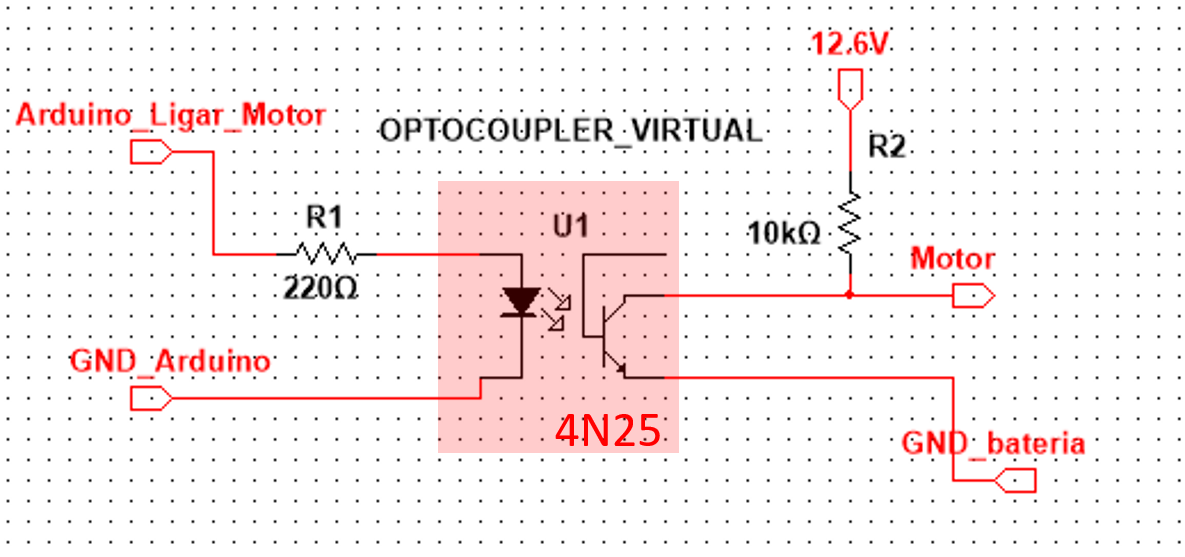
\includegraphics[scale=0.4]{figuras/simulacao_optacoplador.png}
			\caption{Circuito de proteção com acoplamento óptico.}
			\label{img:circuito_de_proteção}
		\end{figure}
	
	% subsection instrumentação (end)

	\subsection{Controle} % (fold)
	\label{sub:controle2}
		O sistema de controle descrito por meio do diagrama de blocos foi implementado utilizando-se os componentes e microcontrolador apresentados na proposta de solução. Abaixo encontra-se o esquemático detalhado do sistema de locomoção e desvio de obstáculos do aspirador. Como explicado anteriormente, foram utilizados quatro sensores ultrassônicos HC-SR04 que posicionam-se a 90º de distância um do outro. Os sensores possuem um ângulo de alcance de 15º e na forma como estão posicionados não cobrem todo o diâmetro do aspirador, no entanto, através de testes experimentais, percebeu-se que a quantidade e distribuição de sensores utilizados, assim como o algoritmo que foi implementado, atendem o requisito de desvio da maior parte dos obstáculos de um cômodo.

		Pode-se observar também no esquemático, o sensor TCRT5000 que foi posicionado na frente da roda boba afim de identificar algum degrau ou desnível que possa impedir o movimento do aspirador ou danificá-lo.

		\begin{figure}[H]
			\centering
			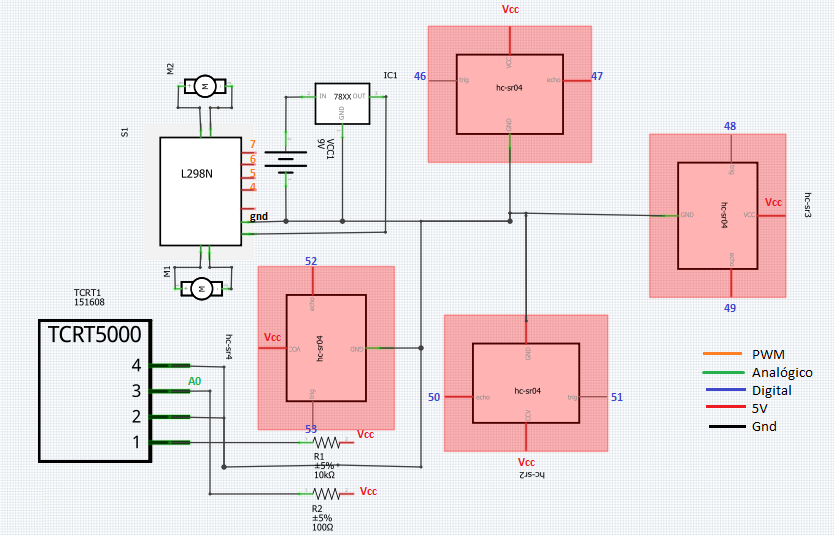
\includegraphics[scale=0.7]{figuras/locomocao1.png}
			\caption{Circuito de locomoção do aspirador.}
			\label{img:circuito_de_locmoção}
		\end{figure}

		Na montagem do circuito utilizou-se entradas analógicas, digitais e PWM. A legenda da figura identifica a natureza dos sinais utilizados de acordo com a pinagem do controlador.

		Os motores são controlados pela ponte H (L298N) que está conectada ao controlador por meio de entradas PWM. A ponte H permite a rotação dos motores nos dois sentidos e o controle de velocidade do mesmo. Sendo assim o aspirador pode se movimentar em todas as direções desviando-se de obstáculos e em uma velocidade adequada para que o sistema de sucção funcione de forma eficiente.

		Durante os testes de locomoção em conjunto com os sensores de obstáculos, observou-se que os sensores ultrassônicos e IR estavam variando muito , atrapalhando assim o movimento do aspirador. Após pesquisas concluiu-se que os motores estavam gerando ruído nos sensores e uma solução encontrada foi utilizar três capacitores cerâmicos de 100nF, um entre as escovas e os outros dois, cada um entre uma escova e a carcaça do motor. O esquema realizado para os dois motores se encontra na figura \ref{img:esquema_de_redução_de_ruido}.

		\begin{figure}[H]
			\centering
			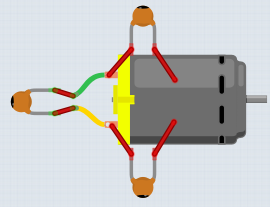
\includegraphics[scale=0.5]{figuras/motorcap.png}
			\caption{Esquema de redução de ruído do motor.}
			\label{img:esquema_de_redução_de_ruido}
		\end{figure}

		O controlador ATMega 2560 controla também o sistema de sucção do aspirador que conta com dois motores. Esse controle foi implementado por meio do chaveamento de transistores. O esquemático apresentado na figura \ref{img:circuito_de_controle_dos_motores} mostra o circuito de controle genérico dos motores do sistema.

		\begin{figure}[H]
			\centering
			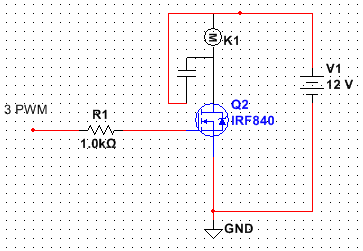
\includegraphics[scale=0.7]{figuras/chave.png}
			\caption{Circuito de controle dos motores.}
			\label{img:circuito_de_controle_dos_motores}
		\end{figure}

		O circuito é ativado por uma saída pwm do controlador que polariza o gate do transistor permitindo que ele conduza corrente através do motor. Por operar com uma corrente alta, utilizou-se um transistor de potência NMOS IRF840 que suporta uma corrente máxima de 8A e 500 V de tensão.

		O motor que ativa o sistema de sucção drena uma corrente muito alta, cerca de 4,4A. Caso haja uma corrente de fuga dos motores para o ATmega, o microcontrolador irá queimar instantaneamente, pois ele suporta até 500mA. Para garantir que essa situação não aconteça, será utilizado um circuito de proteção com optoacopladores, descrito na sessão \ref{sub:Proteção_dos_componentes_2}, que irá isola-lo eletricamente do motor.

	% subsection controle (end)
% section sensoriamento (end)

\subsection{Validação experimental} % (fold)
	\label{sub:validação_experimental}

	APRESENTAR AQUI OS TESTES PARA VALIDAÇÃO.

\section{Comunicação} % (fold)
\label{sec:comunicação2}

	Com o objetivo de detalhar com maior clareza a implementação do sistema de comunicação do projeto, optou-se por utilizar a estratégia \textit{bottom-up}, apresentando toda a especificação técnica dos equipamentos de \textit{hardware} utilizados na solução,seguido da específicação em nível de \textit{Software}.

	\subsection{Hardware} % (fold)
	\label{sub:hardware}
		Um dos requisitos mais críticos do projeto é o da comunicação entre a base e o robô, pois todas as informações colatadas pelo robô são enviadas para a base realizar o processamento, já que a base possui um poder de processamento muito superior ao do próprio robô.

		A implementação do sistema com os \textit{hardwares} especificados na sessão \ref{sub:Hardwar_para_Comunicação} é apresentada na figura \ref{img:hardware_comunicação}.

		\begin{figure}[H]                                                           
      		\centering                    
      		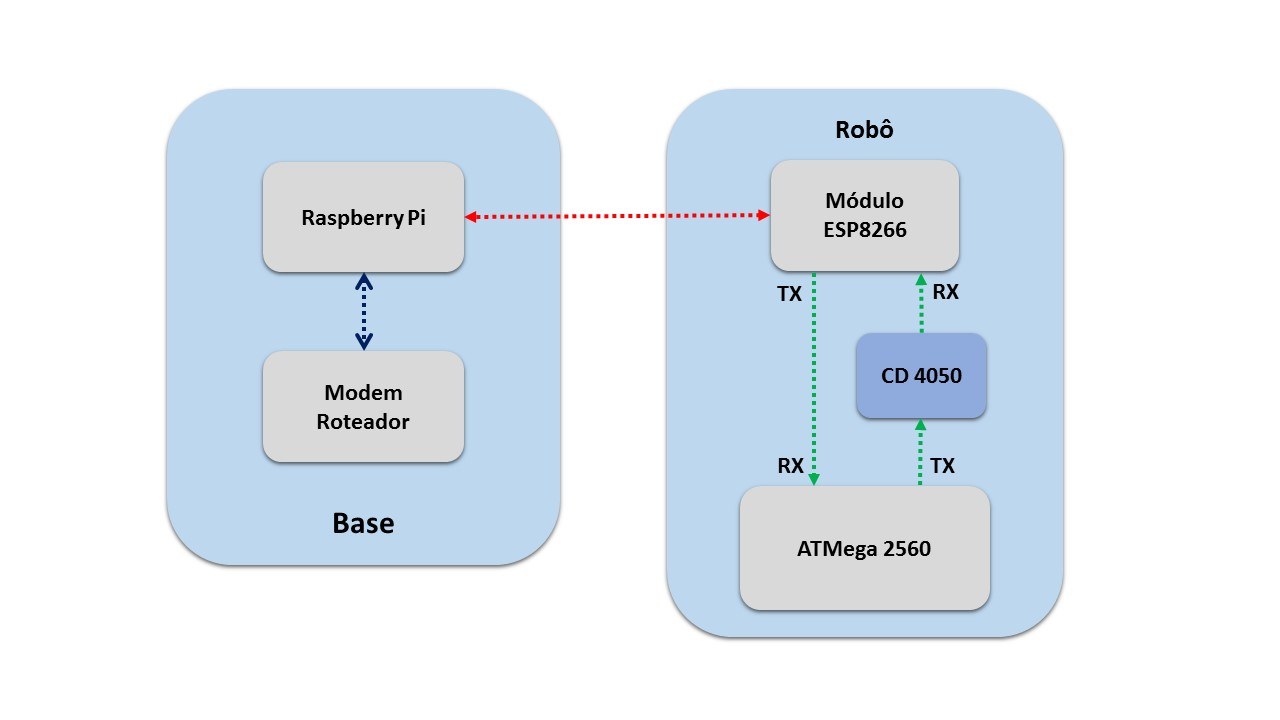
\includegraphics[scale=0.5]{figuras/Hardware_Comunicacao.jpg}               
      		\caption{Esquemático do hardware implementado para realizar a comunicação entre os microprocessadores.}    
      		\label{img:hardware_comunicação}                                            
    	\end{figure}

    	O sistema projetado para a base consiste em um modem roteador conectado a \textit{raspberry pi}, essa conexão é feita por meio de um cabo \textit{ethernet} e dessa forma o sistema é capaz de gerar uma subrede que deve ser acessada pelo robô e pelo usuário quando necessário. A seta vermelha na figura \ref{img:hardware_comunicação} representa essa comunicação entre o robô e a base que é feita via \textit{WiFi} utilizando o protocolo TCP/IP, a seta azul representa a conexão via cabo \textit{ethernet} realizada entre o modem roteador e a \textit{raspberry pi}.

    	Para o robô foi necessário realizar alguns ajustes no projeto inicial que não contemplava o CI CD4050, ao consultar o datasheet do módulo ESP8266 foi constatado que o mesmo trabalha com tensões máximas de ate 3.3V e o controlador utilizado no robô gera sinais com ate 5V, a solução encontrada para resolver esse problema foi utilizar o CI CD4050, que consiste em um buffer não inversor que foi utilizado nesse contexto para converter o nível lógico alto de 5V para 3.3V, a figura \ref{img:datasheet_cd4050} mostra o esquemático interno do CI.

    	\begin{figure}[H]                                                           
      		\centering                    
      		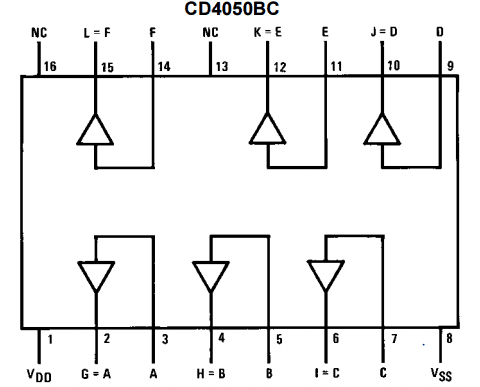
\includegraphics[scale=0.4]{figuras/cd4050.png}               
      		\caption{Esquemático interno do CD4050.(\href{http://www.embarcados.com.br/esp8266-com-arduino/}{Embarcados}})    
      		\label{img:datasheet_cd4050}                                            
    	\end{figure}

    	Por falha de observação, durante a primeira tentativa de montagem desse sistema, acidentalmente foi inserido no RX do módulo uma tensão de 5V, como mencionado anteriormente o módulo trabalha com tensões máximas de 3.3V o que resultou na queima do RX do componente impossibilitando a comunicação serial entre o módulo e o microprocessador, como solução foi adquirido outro módulo igual para continuar o processo de montagem, porem o módulo comprado apresentou falhas na sua inicialização de forma que não foi possível configura-lo da forma desejada, então como última solução foi adquirido um kit de desenvolvimento que garante a correta alimentação exigida pelo ESP8266 facilitando a utilização do mesmo, este foi devidamente configurado de acordo com o projeto e posteriormente será incorporado ao protótipo do projeto, a figura \ref{img:kit_desenvolvimento} apresenta o kit adquirido.

    	\begin{figure}[H]                                                           
      		\centering                    
      		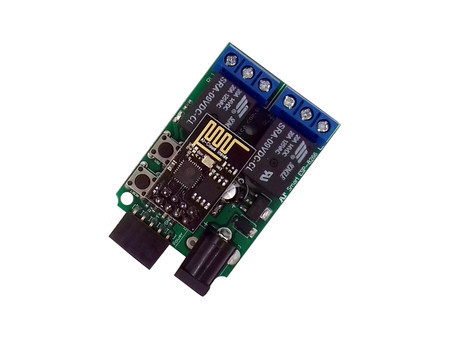
\includegraphics[scale=0.5]{figuras/kit_desenvolvimento.jpg}               
      		\caption{Kit de desenvolvimento ESP8266 \textit{WiFi} 802.11 B/g/n.(\href{http://www.afeletronica.com.br/pd-31421a-esp8266-wifi-802-11-b-g-n-kit-desenvolvimento.html}{AF Eletrônica}})    
      		\label{img:kit_desenvolvimento}                                            
    	\end{figure}

    	Este kit necessita de uma alimentação de 9V/1A, sua alimentação será realizada pela bateria do robô e somente os pinos correspondente ao RX e ao TX serão utilizados pelo microprocessador para realizar a comunicação serial. Essa comunicação serial é representada na figura \ref{img:hardware_comunicação} pelas setas verdes.
	% subsection hardware (end)

	\subsection{Software} % (fold)
	\label{sub:software}
		
		Para realização da comunicação, está sendo utilizado o protocolo de comunicação TCP, enviando e recebendo dados a partir de uma conexão via \textit{sockets} em uma rede criada por um roteador fixo na base. A estratégia de comunicação foi pensada com o objetivo de possibilitar o funcionamento de diversos robôs em uma residência, utilizando a mesma base de processamento. Desse modo, o servidor executado na \textit{raspberry}, em C, aguarda por conexões que podem ser feitas por qualquer cliente que deseje conectar na porta correta (definida neste projeto como 8090).

		Ao identificar uma conexão, uma \textit{thread} é gerada para tratar aquela conexão, entrando em um loop infinito até que o cliente ou o servidor opte por encerrar a conexão. Toda a comunicação realizada entre o robô e a base é feita a partir desta \textit{thread}.

		Quando a \textit{thread} para tratamento da conexão é lançada, a mesma faz a criação de uma nova \textit{thread} que executará paralelamente a ela, que será responsável por enviar comandos ao robô. Ou seja, são criadas duas \textit{threads} para tratar uma mesma conexão, uma \textit{thread} responsável por obter os dados enviados pelo robô e outra responsável por processar estes dados e enviar comandos ao robô.

		Como apenas um canal de comunicação é utilizado, foi necessário utilizar um protocolo que define os padrões de comunicação entre o servidor e o robô. Este protocolo envolve duas partes, onde a primeira representa o \textit{tipo de informação} e a segunda parte representa a \textit{informação} em si. A tabela \ref{tab:protocolo_comunicacao1} apresenta os padrões já definidos e implementados no sistema em relação a comunicação do servidor para o robô.

		\begin{table}[H]
		\centering
		\caption{Padrões de comunicação - Servidor-Robô}
		\label{tab:protocolo_comunicacao1}
		\begin{tabular}{|c|c|}
		\hline
		\multicolumn{2}{|c|}{\textbf{Servidor -\textgreater Robô}} \\ \hline
		\textbf{Padrão}           & \textbf{Descrição}             \\ \hline
		\textit{L 90}             & Virar 90º a esquerda           \\ \hline
		\textit{R 90}                      & Virar 90º a direita            \\ \hline
		\textit{F 10}                      & Andar 10cm a frente            \\ \hline
		\textit{S}                         & Stop                           \\ \hline
		\textit{R}                & Run                            \\ \hline
		\textit{B 10}             & Andar 10cm para trás           \\ \hline
		\textit{B}                & Voltar para base               \\ \hline
		\end{tabular}
		\end{table}

		Já na tabela \ref{tab:protocolo_comunicacao2} estão apresentados os padrões referentes a comunicação do robô para o servidor.

		\begin{table}[H]
		\centering
		\caption{Padrões de comunicação - Robô-Servidor}
		\label{tab:protocolo_comunicacao2}
		\begin{tabular}{|c|c|}
		\hline
		\multicolumn{2}{|c|}{\textbf{Robô -\textgreater Servidor}} \\ \hline
		\textbf{Padrão}        & \textbf{Descrição}                \\ \hline
		\textit{L 90}          & Distância esquerda: 90cm          \\ \hline
		\textit{R 90}                   & Distância direita: 90cm           \\ \hline
		\textit{F 10}                   & Distancia frente: 10cm            \\ \hline
		\textit{B 10}                   & Distancia ré: 10cm            \\ \hline
		\textit{A 45}                   & Bateria 45\%                      \\ \hline
		\textit{P 42}          & Potência do sinal wifi: 42        \\ \hline
		\end{tabular}
		\end{table}

		Com a utilização destes padrões de comunicação, ficou fácil implementar um \textit{porteiro} de cada lado que seja capaz de distribuir as informações para seus respectivos contextos. Esta é a estratégia básica de comunicação entre os dois módulos, mas para isso, uma estrutura foi inicialmente desenvolvida.

		Para realização da comunicação entre os módulos e cliente, faz-se necessário um sistema de autenticação na rede e no sistema de gerenciamento de limpezas. Para isso, foi levantada uma base LDAP de autenticação, utilizando o protocolo RADIUS para conexão na rede. O sistema de gerenciamento de limpezas pode cadastrar novos usuários, incluindo-os na base LDAP, para que o mesmo cadastro realizado no sistema possa ser utilizado para login na rede.

		A arquitetura do sistema, apresentada na seção \ref{sub:arquitetura} registra de maneira clara o funcionamento do sistema de comunicação do projeto. 

	% subsection software (end)

	\subsection{Validação experimental} % (fold)
	\label{sub:validação_experimental}
		
		Com o objetivo de apresentar a realização dos testes e procedimentos relacionados a comunicação do sistema, tanto para o sistema de \textit{Hardware} quanto para \textit{Software}, segue exemplos dos testes realizados para tal.

		\begin{itemize}
			\item \textbf{Comunicação entre módulo ESP8266 e ATMega}

				O teste inicial da comunicação entre o ATMega e o ESP8266 foi realizado utilizando um código que envia ao módulo comandos com o padrão \textit{AT+comando}, ao receber tal comando o módulo deveria responder de acordo com sua programação de fábrica, sendo assim nesse teste foram enviados os comandos \textit{AT+GMR}, \textit{AT+CIFSR} e \textit{AT+CWLAP}. Os retornos esperados pelo ATMega eram, respectivamente, a versão do \textit{firmware}, o \textit{IP} adquirido ao conectar na rede WiFi e uma lista com todas as redes WiFi detectadas.

				Os resultados desse teste estão apresentados na figura \ref{img:teste_arduino_modulo}, o código utilizado para esse teste esta disponível em \href{https://github.com/kaiocoelho/CodigoESP/blob/master/codigo_teste/codigo_teste_inicial.ino}{Teste ESP8266}.

				\begin{figure}[H]                                                           
			  		\centering                    
			  		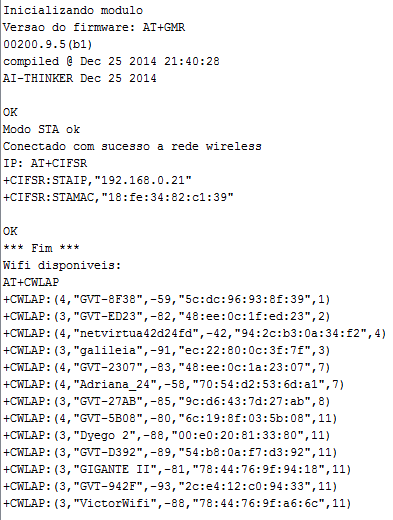
\includegraphics[scale=0.9]{figuras/testeModuloWifi}               
			  		\caption{Teste de comunicação Arduino/módulo Wifi.}    
			  		\label{img:teste_arduino_modulo}                                            
				\end{figure}

			\item \textbf{Comunicação entre ATMega e Raspberry Pi}

				Com a comunicação concluída entre o Arduino e o Módulo Wifi, é possível trabalhar em um nível de abstração maior, partindo para a lógica de software e comunicação do sistema. Tendo acesso a rede wifi, foi possível implementar uma comunicação via TCP/IP, utilizando o protocolo de comunicação apresentado nas tabelas \ref{tab:protocolo_comunicacao1} e \ref{tab:protocolo_comunicacao2}.		

				Na Figura \ref{img:dois_lados_comunicacao}, é apresentada a comunicação sendo feita entre o Arduino e a Raspberry, onde o Arduino envia informações sobre 3 sonares, a raspberry processa essas informações e retorna os comandos necessários para desviar de obstáculos e se locomover pelo ambiente.

				\begin{figure}[H]                                                           
			  		\centering                    
			  		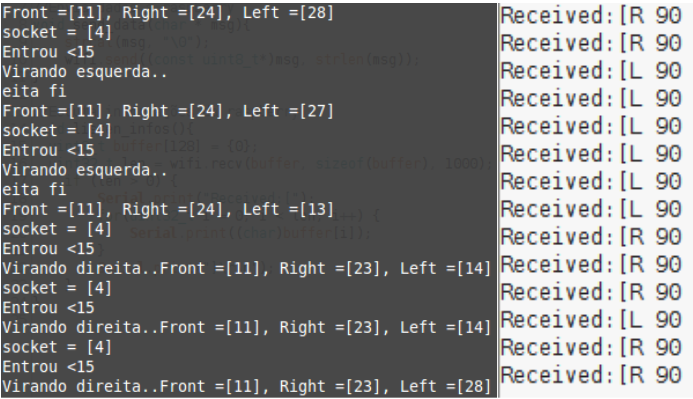
\includegraphics[scale=0.4]{figuras/teste_arduino_rasp}               
			  		\caption{Teste de comunicação Arduino/Raspberry.}    
			  		\label{img:dois_lados_comunicacao}                                            
				\end{figure}

		\end{itemize}
	% subsection validação_experimental (end)
% section comunicação (end)

\section{Interface} % fold
\label{sub:interface}
  Para a realização da interface com o usuário, foi criado uma aplicação web, utilizando o \textit{framework} livre, Ruby on Rails\cite{rails}.
Esse \textit{framework} permite desenvolvimento de sites e usa como linguagem o Ruby. Sua arquitetura padrão é o MVC(\textit{Model-View-Controller}),
 que basicamente separa a aplicação em 3 camadas. A camada de interação do usuário(\textit{view}), a camada de manipulação dos dados(\textit{model}) 
e a camada de controle(\textit{controller})\cite{mvc}.
  O rails permite adicionar bibliotecas com funções especias, essas bibliotecas tem o nome de \textit{gem}. Para nossa aplicação, além das gems já padrões para a utilização
  do rails, também utilizamos as gems que podem ser vistas na tabela \ref{gems}.
\begin{table}[H]
\centering
\caption{Gems}
\label{gems}
\begin{tabular}{|l|l|}
\hline
\rowcolor[HTML]{C0C0C0} 
{\color[HTML]{333333} \textbf{Gem}} & {\color[HTML]{333333} \textbf{Descrição}} \\ \hline
devise\_ldap\_authenticatable       & Para autenticar junto com uma base LDAP   \\ \hline
cancancan                           & Para autorização                          \\ \hline
rolify                              & Para criar funções de usuários            \\ \hline
fullcalendar-rails                  & Para mostrar calendário de agendamento    \\ \hline
momentjs-rails                      & Auxílio ao calendário                     \\ \hline
bootstrap-sass                      & Para layout das páginas                   \\ \hline
rails-erd                           & Para gerar diagrama de classe             \\ \hline
\end{tabular}
\end{table}

A figura \ref{img:diagrama} mostra o diagrama de domínio do projeto

\begin{figure}[H]
	\centering
	\includegraphics[scale=0.7]{figuras/erd.pdf}
	\caption{Diagrama de domínio.}
	\label{img:diagrama}
\end{figure}

A classe \textit{User} foi criada para realizar o login na aplicação, sendo utilizada em conjunto com a \textit{gem} devise\_ldap\_authenticable. Ela possui um relacionamento com a classe \textit{Role} que atribui uma função ao usuário. Atualmente, só está sendo utilizado a função de administrador. Por fim, a classe Agenda é responsável por guardar os agendamentos feitos pelo usuário. O código da interface do R2-PI2 está no \href{https://github.com/PI2Aspirador/railsApp}{Github}.

As imagens a seguir mostram como está a interface.

\begin{figure}[H]
	\centering
	\includegraphics[scale=0.3]{figuras/home_interface.png}
	\caption{Interface - Home.}
	\label{img:home}
\end{figure}

\begin{figure}[H]
	\centering
	\includegraphics[scale=0.3]{figuras/login.png}
	\caption{Interface - Login.}
	\label{img:login}
\end{figure}

\begin{figure}[H]
	\centering
	\includegraphics[scale=0.3]{figuras/agendamento.png}
	\caption{Interface - Agendamento.}
	\label{img:agendamento}
\end{figure}


\section{Arquitetura do Sistema de Software} % (fold)
\label{sub:arquitetura}

Em relação a arquitetura do sistema, a mesma foi definida em módulos, contemplando 5 módulos distribuídos. A comunicação entre os principais módulos é feita a partir da utilização de \textit{sockets} por conexão TCP. De modo geral, a arquitetura pode ser representada pela Figura \ref{img:arquitetura}.

\begin{figure}[H]
	\centering
	\includegraphics[scale=0.7]{figuras/diagrama_arquitetural.png}
	\caption{Diagrama arquitetural do sistema R2-PI2.}
	\label{img:arquitetura}
\end{figure}

O \textit{Servidor Tempo Real} gerencia diversas \textit{threads} para processar e instruir informações ao robô. O escalonamento destas \textit{threads} segue o padrão de sistemas em tempo real, a partir da configuração do \textit{patch RT\_Preempt} no Kernel utilizado no servidor. Desse modo, o tempo de resposta a requisições advindas do robô é otimizado, buscado evitar falhas de controle relacionadas ao atraso do sistema.

A comunicação entre Robô e Servidor Tempo Real segue uma arquitetura cliente-servidor, onde o cliente e o servidor acabam trocando de papéis em determinadas ocasiões. Em alguns instantes o robô fará requisições ao servidor, que lhe retorna uma resposta, já em outros instantes o servidor fará requisições ao robô, obtendo também uma resposta. 

O principal motivo da escolha desta arquitetura se refere ao poder de processamento presente no servidor, em relação ao processamento encontrado no robô (ATMega). Como o sistema é caracterizado como um sistema de tempo real, necessitou-se da utilização deste mecanismo de processamento.

Como interface do sistema para o cliente, foi desenvolvido o sistema Gestor de Limpezas, em rails. Este sistema faz comunicação com o Sistema Tempo Real e a base de registro de usuários (LDAP). Neste sistema é possível agendar limpezas, iniciar e parar uma limpeza e análisar \textit{status} de limpeza. A comunicação entre os dois sistemas é feita a partir de sockets locais, já que os dois serão executados na mesma máquina (raspberry pi).

\section{Plano de integração e validação} % (fold)
\label{sec:plano_de_integração_e_validação}
	Após implementar os subsistemas é necessário planjear a maneira como será realizada a integração entre eles, as figuras \ref{img:integração_robô} e \ref{img:integração_base} apresentam de maneira geral as relações existentes entre os subsistemas de acordo com as implmementações realizadas.

	\begin{figure}[H]                                                           
   		\centering                                                                
   		\includegraphics[scale=0.5]{figuras/plano_integracao_robo.jpg}               
   		\caption{Plano geral de integração dos subsistemas par ao robô.}    
   		\label{img:integração_robô}                                            
   	\end{figure} 

   	\begin{figure}[H]                                                           
   		\centering                                                                
   		\includegraphics[scale=0.5]{figuras/plano_integracao_base.jpg}               
   		\caption{Plano geral de integração dos subsistemas para a base.}    
   		\label{img:integração_base}                                            
   	\end{figure} 

   	\noindent \textbf{Legenda}: \\
   	\noindent \textit{Setas de cor verde} - simbolizam que determinado bloco tem controle sobre um outro bloco. \\
   	\noindent \textit{Setas de cor laranja} - simbolizam a allimentação necessária para os componentes. \\
   	\noindent \textit{Setas de cor cinza} - simbolizam que há comunicação entre os blocos (os sentidos das setas indicam os caminhos dos dados).

\subsection{Testes de validação do plano de integração}
\label{sub:validação_plano_integração}
   \subsubsection{Sistema de Sucção}
   \begin{enumerate}
      \item \textbf{Alimentar o aspirador com a bateria e testar a eficácia de aspiração de partículas}

         O aspirador ao ser ligado a bateria obteve uma boa sucção, assim como nos testes de bancada. Entretanto, depois de alguns minutos ligados, a bateria começa a perder diferença de potencial, fazendo com que o aspirador comece a perder eficiência. Após 12 minutos, a bateria já não possuía tensão para manter o sistema funcionando de forma eficiente. Constatou-se também uma alta temperatura nas baterias. 

      \item \textbf{Alimentar o motor escova e garantir que ele esteja rodando}

         A alimentação foi suficiente para garantir a rotação do motor. Verificou-se que após um tempo grande de funcionamento, o temperatura do motor amolece a cola utilizada para sua fixação. Durante os testes com a escova, o motor DC utilizado teve um travamento repentino do eixo. Acredita-se que parte da sujeira entrou no motor, causando o seu travamento completo. 

      \item \textbf{Testar os transistores do motor da escova e do aspirador}

         Não foi possível realizar esse teste devido ao mal funcionamento das baterias. 

      \item \textbf{Testar o sinal de controle do arduino até os transistores}

         Não foi possível realizar esse teste devido ao mal funcionamento das baterias. 

      \item \textbf{Ligar a aspiração e a escova com o sistema funcionando em 100\%}

         Esse teste não foi realizado devido ao mal funcionamento que ocorreu nas novas baterias adquiridas. No dia do teste de integração, o aspirador funcionou individualmente. Mas ao conectar o aspirador ao resto do sistema, nenhum componente do sistema ligou. Depois de analisar cuidadosamente para identificar o problema, constatou-se que a bateria não fornecia tensão nem corrente.  

   \end{enumerate}

   \subsection{Modificações realizadas após os testes}
   \label{sub:mudanças}
   \begin{itemize}
      \item Troca do motor da escova:

         Devido ao travamento do motor da escova, foi necessário realizar a troca do mesmo. O novo motor DC colocado possui 9V de tensão nominal e 0.5 A de corrente nominal quando o eixo está carregado.

         \begin{figure}[H]                                                           
            \centering                                                                
            \includegraphics[scale=0.5]{figuras/SuccaoPC3_1.jpg}               
            \caption{Teste de coleta de sujeira com o novo motor acoplado.}    
            \label{img:teste_coleta}                                            
         \end{figure} 

      \item Troca dos cabos do aspirador e da escova:

         Foram adicionados cabos mais grossos e resistentes devido a quantidade de corrente que está sendo utilizada no circuito. 

      \item Acréscimo de mais pano na escova:

         Foi adicionado mais pano a escova com o objetivo de aumentar a eficiência do sistema de sucção. O pano adicionado garante que a sujeira seja varrida e contida ao alcance das cerdas da escova, de forma a garantir mais tempo para o sistema coletar a sujeira.

         \begin{figure}[H]                                                           
            \centering                                                                
            \includegraphics[scale=0.5]{figuras/SuccaoPC3_2.jpg}               
            \caption{Teste de coleta de sujeira após o acréscimo de pano a escova.}    
            \label{img:teste_coleta_pano}                                            
         \end{figure} 

      \item Modificação estrutural interna da escova

         Foi aberto um vão na parte interna da escova que fica próxima ao cano do aspirador. Essa modificação aumentou drasticamente a eficiência na coleta de sujeira por parte da escova.

         \begin{figure}[H]                                                           
            \centering                                                                
            \includegraphics[scale=0.5]{figuras/SuccaoPC3_3.jpg}               
            \caption{Teste da coleta de sujeira com a abertura de parte da parede interna.}    
            \label{img:teste_coleta_sujeira}                                            
         \end{figure}

      \item Troca da mangueira do aspirador:

         A mangueira antiga utilizada no aspirador era sanfonada, o que prejudica o desempenho do aspirador. Foi adicionada uma mangueira de borracha com superfície interna lisa, com o objetivo de diminuir a perda de carga do sistema.  

         \begin{figure}[H]                                                           
            \centering                                                                
            \includegraphics[scale=0.5]{figuras/SuccaoPC3_4.jpg}               
            \caption{Imagem dos novos cabos e da nova mangueira ligada ao aspirador.}    
            \label{img:novo_sistema_sucção}                                            
         \end{figure}

   \end{itemize}
% section plano_de_integração_e_validação (end)
